\chapter{OUTPUT REGULATION PARA SEGUIMIENTO A SEÑALES SINUSOIDALES}
\label{cap:OutputRegulation}
\markboth{CAPÍTULO \thechapter. OUTPUT REGULATION}{CAPÍTULO \thechapter. OUTPUT REGULATION}

En este capítulo se resuelve la problemática del seguimiento sinusoidal para la plataforma Stewart. Para esto se desarrolla un nuevo controlador basado en los controladores MIMO PID obtenidos en el capítulo \ref{cap:mimoPID} anterior sintetizados mediante diseño de control LQI. Mediante el principio del modelo interno se obtiene una solución estable para esta problemática. Los resultados del controlador son simulados y comparados mediante tablas bajo distintos índices de desempeño. 

Para modo de simplificación, en el diseño de los controladores con Output Regulation y simulaciones respectivas, la referencia asignada en este capítulo \ref{cap:OutputRegulation} sera con respecto a la posición de los brazos $l(t)$ específicamente. No se considerará el movimiento de la plataforma superior $q_{ref}(t)$ como referencia para este capítulo. 

Se considerarán 2 casos de referencias sinusoidales, la primera referencia de igual señal sinusoidal para todos los brazos de la plataforma (misma amplitud, frecuencia y fase), mientras que la segunda referencia poseerá distintas señales sinusoidales para cada brazo.

\newpage
\section{Diseño control LQR con Output Regulation para referencias sinusoidales de única frecuencia}
\lhead[\thepage]{Sección \thesection. LQR Output Regulation frecuencia única}
\label{sec:LQR_outputRegulation_frec_fija}

Se considera el sistema linealizado \ref{eq:sys_varestados_transf} con la transformación de similaridad de la plataforma Stewart, desarrollado en la sección \ref{sec:linealizacion_stewart} del Capítulo \ref{cap:modeladoStewart}. Recordando las ecuaciones del sistema:

\begin{subequations} \label{eq:sysStewart_outputregulation}
    \begin{align}
        \Dot{\xi}(t) & = A_0 \cdot \xi(t) + B_0 \cdot u(t), \\
        y(t) & = C_0 \cdot \xi(t) + D_0 \cdot u(t)
    \end{align}    
\end{subequations}
con los estados internos
\begin{align} 
    \xi (t) & = \begin{bmatrix}
        l(t)^{\top} & \dot{l}(t)^{\top}
    \end{bmatrix}^{\top} \notag \\
    & = \begin{bmatrix}
        l_1(t) & \hdots & l_6(t) & \dot{l}_1(t) & \hdots & \dot{l}_6(t)
    \end{bmatrix}^{\top}
\end{align}

Como $C_0 = I_{12\times12}$ y $D_0 = 0$ se obtiene como medición directa de la plataforma los estados internos del sistema correspondientes a la posición y velocidad de los brazos. \\

Se define la nueva referencia sinusoidal para el diseño de control LQR con Output Regulation. Esta referencia se caracteriza por modelar la posición de los brazos (no velocidad), además de poseer una frecuencia $\theta$, fase $\phi$ y amplitudes $\Upsilon_{sin}$ $\Upsilon_{step}$ iguales para cada brazo:

\begin{equation}
    l_{ref}(t) = \begin{bmatrix}
        \Upsilon_{sin} sin(\theta t + \phi) + \Upsilon_{step}\\
        \Upsilon_{sin} sin(\theta t + \phi) + \Upsilon_{step}\\
        \Upsilon_{sin} sin(\theta t + \phi) + \Upsilon_{step}\\
        \Upsilon_{sin} sin(\theta t + \phi) + \Upsilon_{step}\\
        \Upsilon_{sin} sin(\theta t + \phi) + \Upsilon_{step}\\
        \Upsilon_{sin} sin(\theta t + \phi) + \Upsilon_{step}\\
    \end{bmatrix}
\end{equation}

Se transforma la referencia de los 6 brazos como sistema independiente exógeno tal como se explica en el problema de Output Regulation de la sección \ref{sec:outputregulation} del Capítulo \ref{cap:Notación y preliminares}. 

Para este caso, el sistema exógeno de la referencia estará formado por 3 estados internos correspondientes a un escalón, una sinusoidal y su derivada, de la forma $v(t)=\begin{bmatrix} step & sin & \frac{d}{dt}(sin) \end{bmatrix}$. Mediante esta representación es posible formar cualquier referencia compuesta por señales escalón y sinusoidal.
\begin{align}
\label{eq:sys_ref_fija}
    \dot{v}(t) & = H_v v(t), \notag \\
    l_{ref}(t) & = C_v v(t)
\end{align}
donde 
\begin{gather}
    \begin{align}
    H_v & = \begin{bmatrix}
        H_{v1} & \hdots & 0 \\
        \vdots & \ddots & \vdots \\ 
        0 & \hdots & H_{v6}
    \end{bmatrix}, 
    \quad \textrm{con } \quad
    H_{vi} = \begin{bmatrix}
        0 & 0 & 0 \\
        0 & 0 & 1 \\
        0 & -\theta^2 & 0
    \end{bmatrix}, \notag \\
    C_v & = \begin{bmatrix}
        C_{v1} & \hdots & 0 \\
        \vdots & \ddots & \vdots \\ 
        0 & \hdots & C_{v6}
    \end{bmatrix},
    \quad \textrm{con } \quad
    C_{vi} = \begin{bmatrix}
        \Upsilon_{step} & \Upsilon_{sin} & 0
    \end{bmatrix},
    \end{align} \\
    v(0) = \begin{bmatrix}
        \begin{bmatrix} 1 & sin(\phi) & \theta cos(\phi) \end{bmatrix} & \hdots & \begin{bmatrix} 1 & sin(\phi) & \theta cos(\phi) \end{bmatrix} 
    \end{bmatrix}_{1\times18}, \quad 
    \textrm{tal que } i = 1,\hdots,6 \notag
\end{gather}

La importancia del sistema exógeno anterior, es que la matriz $H_v$ posee la información de la frecuencia de cada sinusoidal que se desea seguir en cada brazo. 

Una vez desarrollada la referencia deseada, se procede a diseñar el controlador LQR el cual sera la base para el desarrollo del Output Regulation. 

Tal como se define en la sección \ref{sec:lqicontrol} del Capítulo \ref{cap:Notación y preliminares}, se obtiene mediante el Lema \ref{lem1:riccati_infinto} la matriz de realimentación $K_\xi$ del control LQR, encargada de regular los estados internos del sistema \ref{eq:sysStewart_outputregulation} de interés (debe tener incluido el signo negativo propio del control LQR).

Con $K_\xi$ obtenido, se procede a resolver la matriz solución $K_v$ de Output Regulation mediante el Teorema \ref{teo1:OutputRegulation} de la sección \ref{sec:outputregulation} del capítulo \ref{cap:Notación y preliminares}. Se resuelve $X$ y $U$ del sistema de ecuaciones reguladoras (demostrado en Apéndice \ref{appen1}) caracterizado en este caso por: la matriz $H_v$ de los estados de la referencia, la matriz $C_v$ de la referencia deseada y las matrices $A_0, B_0, C_{pos}, D_0$ de la plataforma propiamente tal (como no se tiene ruido en el sistema, entonces $E=0$ y $F=-C_v$ del Teorema \ref{teo1:OutputRegulation}):
\begin{align} \label{eq:OR_equations_fija}
    X H_v = A_0 X + B_0 U \notag \\
    0 = C_{pos} X + D_0 U - C_v 
\end{align}

\begin{remark}
Como se esta regulando unicamente posición de brazos en la referencia, se debe utilizar en las ecuaciones la matriz $C_{pos}=\begin{bmatrix}I_{6\times6} & 0_{6\times6}\end{bmatrix}$ en vez de $C_0$ de la plataforma, para así regular solo posición sin agregar la medición de velocidad disponible.
\end{remark}

Con $X$ y $U$ obtenidos, se despeja $K_v$ desde la igualdad $K_v = U - K_\xi X$.

Finalmente, se obtiene la ley de control final utilizada para el control LQR con Output Regulation de la plataforma Stewart, constituida por una matriz de realimentación $K_\xi$ de los estados internos de la plataforma, junto con una matriz feedforward $K_v$ de los estados de la referencia deseada:

\begin{equation} \label{eq:OR_law_control_fija}
    u(t) = K_\xi \xi(t) + K_v v(t)
\end{equation}






\section{Diseño control LQR con Output Regulation para referencias sinusoidales de distinta amplitud, frecuencia y fase}
\lhead[\thepage]{Sección \thesection. LQR Output Regulation frecuencia variada}

Considerando el mismo sistema linealizado \ref{eq:sysStewart_outputregulation} de la plataforma Stewart, se redefine la referencia deseada diferenciando en amplitud, frecuencia y fase entre cada trayectoria:

\begin{equation}
    l_{ref}(t) = \begin{bmatrix}
        \Upsilon_{sin1} sin(\theta_1 t + \phi_1) + \Upsilon_{step1}\\
        \Upsilon_{sin2} sin(\theta_2 t + \phi_2) + \Upsilon_{step2}\\
        \Upsilon_{sin3} sin(\theta_3 t + \phi_3) + \Upsilon_{step3}\\
        \Upsilon_{sin4} sin(\theta_4 t + \phi_4) + \Upsilon_{step4}\\
        \Upsilon_{sin5} sin(\theta_5 t + \phi_5) + \Upsilon_{step5}\\
        \Upsilon_{sin6} sin(\theta_6 t + \phi_6) + \Upsilon_{step6}\\
    \end{bmatrix}
\end{equation}

Se define el nuevo sistema exógeno, que posee una diferenciación de frecuencia, amplitud y fase a cada trayectoria deseada de cada brazo. 

\begin{align}
\label{eq:sys_ref_variable}
    \dot{v}(t) & = H_v v(t), \notag \\
    l_{ref}(t) & = C_v v(t)
\end{align}
donde 
\begin{gather}
    \begin{align}
    H_v & = \begin{bmatrix}
        H_{v1} & \hdots & 0 \\
        \vdots & \ddots & \vdots \\ 
        0 & \hdots & H_{v6}
    \end{bmatrix}, 
    \quad \textrm{con } \quad
    H_{vi} = \begin{bmatrix}
        0 & 0 & 0 \\
        0 & 0 & 1 \\
        0 & -\theta_i^2 & 0
    \end{bmatrix}, \notag \\
    C_v & = \begin{bmatrix}
        C_{v1} & \hdots & 0 \\
        \vdots & \ddots & \vdots \\ 
        0 & \hdots & C_{v6}
    \end{bmatrix},
    \quad \textrm{con } \quad
    C_{vi} = \begin{bmatrix}
        \Upsilon_{step\textrm{ }i} & \Upsilon_{sin\textrm{ }i} & 0
    \end{bmatrix}, 
    \end{align} \\
    v(0) = \begin{bmatrix}
        \begin{bmatrix} 1 & sin(\phi_1) & \theta_1 cos(\phi_1) \end{bmatrix} & \hdots & \begin{bmatrix} 1 & sin(\phi_6) & \theta_6 cos(\phi_6) \end{bmatrix} 
    \end{bmatrix}, \quad
    \textrm{tal que } i = 1,\hdots,6 \notag
\end{gather}

Después de redefinir la referencia, con las matrices del sistema lineal \ref{eq:sysStewart_outputregulation} se obtiene la matriz de realimentación LQR denominada $K_\xi$ mediante el Lema \ref{lem1:riccati_infinto}, que en este caso es igual a la sección anterior (con signo negativo incluido del control LQR).

Con esta matriz $K_\xi$, se resuelve el mismo sistema de ecuaciones \ref{eq:OR_equations_fija} para $X$ y $U$ (Teorema \ref{teo1:OutputRegulation}), con la nueva matriz de referencia $H_v$ que incluye diferenciación en frecuencia y las matrices del sistema lineal junto a $C_{pos}$ para medir solo posición de la planta. 

Con $X$ y $U$ obtenidos se despeja $K_v$ desde la igualdad $K_v = U - K_\xi X$.

Finalmente se obtiene la misma ley de control \ref{eq:OR_law_control_fija} LQR con Output Regulation para referencias sinusoidales de distintas frecuencias, con $K_\xi$ la matriz estabilizante de los estados internos de la planta y $K_v$ la matriz feedforward de los estados de la referencia. 


%###############################################
%###############################################
%###############################################
\section{Resultados de simulación control LQR con Output Regulation}
\lhead[\thepage]{Sección \thesection. Resultados de simulación LQR con Output Regulation}

Para el control LQR con Output Regulation se utiliza el esquema de control mostrado en la Figura \ref{fig:lqr_OR_stewart_scheme}. Se puede apreciar claramente la matriz de realimentación $K_\xi$ encargada de regular los estados internos del sistema, junto a la matriz feedforward $K_v$ para el seguimiento a la referencia.

\begin{figure}[ht]
\centering
    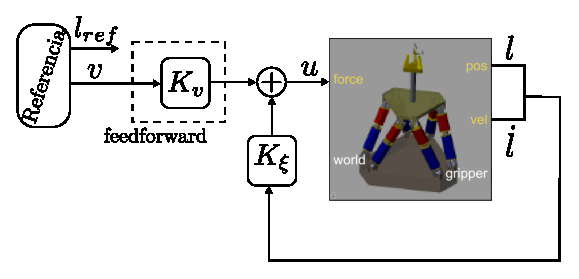
\includegraphics[width=0.7\columnwidth]{Figures/Output_Regulation/lqr_OR_stewart_scheme.eps}
    \caption{Esquema de control LQR con Output Regulation para la plataforma Stewart.}
    \label{fig:lqr_OR_stewart_scheme}
\end{figure}


Se utilizan las matrices $A_0, B_0, C_0, D_0$ del sistema lineal \ref{eq:sysStewart_outputregulation} de la plataforma Stewart.

Con las matrices del sistema lineal, se obtiene la matriz de realimentación $K_\xi$ (con signo negativo incluido) de los estados internos del sistema mediante el Lema \ref{lem1:riccati_infinto}:

\begin{equation}
    K_\xi = \scalebox{0.8}{$\begin{bmatrix}
        \textrm{-}13.433 &	6.858 &	2.100 &	\textrm{-}4.205 &	1.542 &	3.748 &	\textrm{-}3.844 &	0.547 &	0.281 &	\textrm{-}0.394 &	0.120 &	0.087 \\
        6.865 &	\textrm{-}13.400 &	3.743 &	1.520 &	\textrm{-}4.198 &	2.080 &	0.545 &	\textrm{-}3.842 &	0.088 &	0.118 &	\textrm{-}0.393 &	0.280 \\
        1.518 &	3.788 &	\textrm{-}13.476 &	6.865 &	2.098 &	\textrm{-}4.200 &	0.119 &	0.088 &	\textrm{-}3.845 &	0.547 &	0.281 &	\textrm{-}0.395 \\
        \textrm{-}4.176 &	2.117 &	6.856 &	\textrm{-}13.494 &	3.796 &	1.514 &	\textrm{-}0.395 &	0.282 &	0.548 &	\textrm{-}3.846 &	0.089 &	0.119 \\
        2.148 &	\textrm{-}4.157 &	1.495 &	3.787 &	\textrm{-}13.506 &	6.846 &	0.283 &	\textrm{-}0.396 &	0.118 &	0.089 &	\textrm{-}3.847 &	0.548 \\
        3.774 &	1.497 &	\textrm{-}4.192 &	2.101 &	6.875 &	\textrm{-}13.460 &	0.088 &	0.118 &	\textrm{-}0.395 &	0.282 &	0.547 &	\textrm{-}3.845 
    \end{bmatrix}$}
\end{equation}

%--------------------------------------------------
\newpage
\subsection{Referencia sinusoidal Nro.1 frecuencia fija}

Se define la referencia Nro.1 a seguir de cada brazo actuador de la plataforma Stewart, caracterizada por un escalón y sinusoidales de misma amplitud, frecuencia y fase para todos los brazos: 
\begin{equation}
    l_{ref1}(t) = \begin{bmatrix}
        2 sin(\pi t) + 10\\
        2 sin(\pi t) + 10\\
        2 sin(\pi t) + 10\\
        2 sin(\pi t) + 10\\
        2 sin(\pi t) + 10\\
        2 sin(\pi t) + 10\\
    \end{bmatrix}
\end{equation}

Se establecen así los parámetros de la referencia:
\begin{itemize}
    \item amplitud escalón $\Upsilon_{step}=10$.
    \item amplitud sinusoidal $\Upsilon_{sin}=2$, \\
    frecuencia $\theta=\pi$, \\
    fase $\phi=0$.
\end{itemize}

Con los parámetros obtenidos de la referencia se modela su sistema exógeno de \ref{eq:sys_ref_fija}. Con el sistema exógeno de la referencia y los parámetros del sistema \ref{eq:sysStewart_outputregulation} de la plataforma Stewart, se obtiene la matriz feedforward $K_v$ del control para la referencia sinusoidal Nro.1:

\begin{multline}
    K_v = \scalebox{0.75}{$\left[\begin{matrix}
        73.878 &	12.138 &	7.689 &	\textrm{-}29.820 &	\textrm{-}4.249 &	\textrm{-}1.094 &	\textrm{-}10.957 &	\textrm{-}1.612 &	\textrm{-}0.562 &	20.854 &	3.267 &	0.789 \\
        \textrm{-}29.762 &	\textrm{-}4.237 &	\textrm{-}1.091 &	73.682 &	12.099 &	7.685 &	\textrm{-}17.338 &	\textrm{-}3.586 &	\textrm{-}0.175 &	\textrm{-}4.819 &	\textrm{-}0.384 &	\textrm{-}0.237 \\
        \textrm{-}4.844 &	\textrm{-}0.389 &	\textrm{-}0.238 &	\textrm{-}17.338 &	\textrm{-}3.586 &	\textrm{-}0.175 &	73.946 &	12.152 &	7.691 &	\textrm{-}29.876 &	\textrm{-}4.260 &	\textrm{-}1.095 \\
        20.906 &	3.277 &	0.791 &	\textrm{-}11.006 &	\textrm{-}1.621 &	\textrm{-}0.564 &	\textrm{-}29.907 &	\textrm{-}4.266 &	\textrm{-}1.096 &	74.108 &	12.184 &	7.693 \\
        \textrm{-}11.177 &	\textrm{-}1.656 &	\textrm{-}0.567 &	20.881 &	3.272 &	0.792 &	\textrm{-}4.822 &	\textrm{-}0.385 &	\textrm{-}0.236 &	\textrm{-}17.541 &	\textrm{-}3.626 &	\textrm{-}0.179 \\
        \textrm{-}17.347 &	\textrm{-}3.588 &	\textrm{-}0.177 &	\textrm{-}4.740 &	\textrm{-}0.368 &	\textrm{-}0.236 &	20.868 &	3.270 &	0.790 &	\textrm{-}11.063 &	\textrm{-}1.633 &	\textrm{-}0.563 \\
    \end{matrix}\right.$} \\
    \scalebox{0.75}{$\left. \begin{matrix}
        \textrm{-}4.997 &	\textrm{-}0.420 &	\textrm{-}0.240 &	\textrm{-}17.298 &	\textrm{-}3.578 &	\textrm{-}0.174 \\
        20.750 &	3.246 &	0.786 &	\textrm{-}10.849 &	\textrm{-}1.590 &	\textrm{-}0.559 \\
        \textrm{-}10.985 &	\textrm{-}1.617 &	\textrm{-}0.562 &	20.859 &	3.268 &	0.789 \\
        \textrm{-}17.514 &	\textrm{-}3.621 &	\textrm{-}0.177 &	\textrm{-}4.902 &	\textrm{-}0.401 &	\textrm{-}0.237 \\
        74.255 &	12.214 &	7.695 &	\textrm{-}29.912 &	\textrm{-}4.267 &	\textrm{-}1.096 \\
        \textrm{-}29.848 &	\textrm{-}4.255 &	\textrm{-}1.093 &	73.887 &	12.140 &	7.689 \\
    \end{matrix}\right]$}
\end{multline}



\subsubsection{Simulación Sistema Lineal}

En la Figura \ref{fig:lqrOR_lineal_frec_fija} se puede apreciar el error de seguimiento de los brazos actuadores del sistema lineal. Como se puede notar, el efecto del Output Regulation funciona perfectamente al seguir a la referencia sinusoidal de frecuencia única, mostrando un error cero en estado estacionario para el sistema linealizado.

\begin{figure}[H]
\centering
    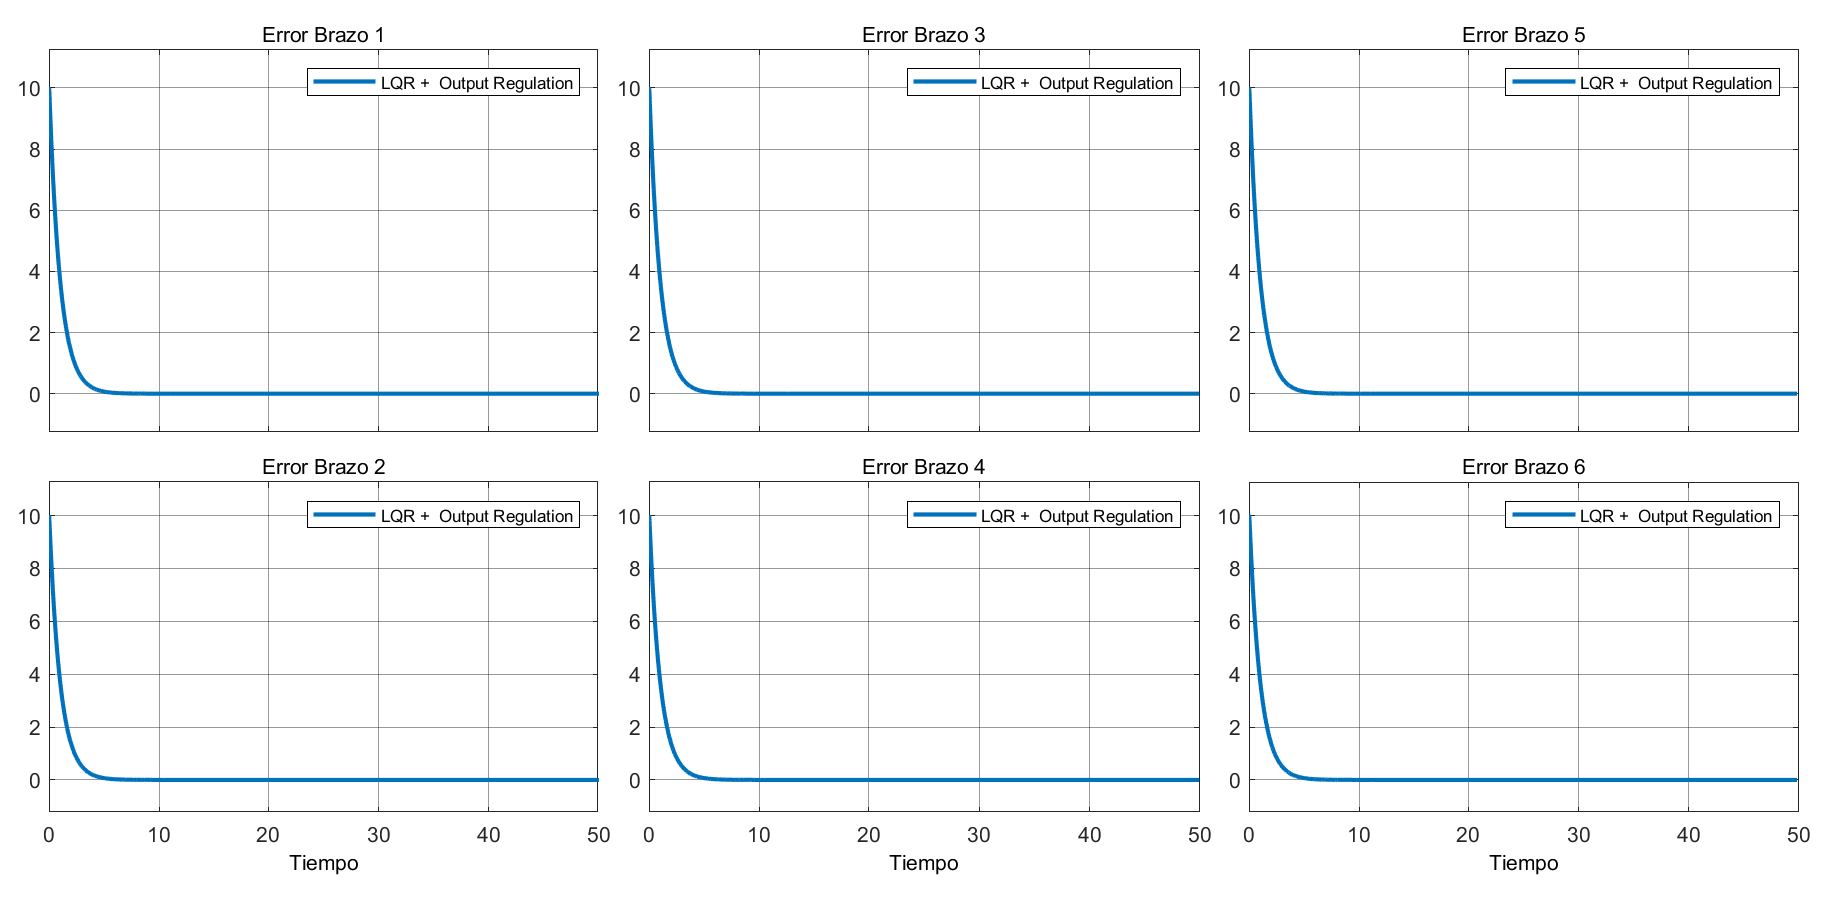
\includegraphics[width=0.9\columnwidth]{Results/lqrOR_frec_fija/lqr_sys_lineal_frec_fija.eps}
    \caption{Error de seguimiento (cm) LQR + Output Regulation sistema lineal, referencia frecuencia fija.}
    \label{fig:lqrOR_lineal_frec_fija}
\end{figure}

\subsubsection{Simulación Sistema No-Lineal}

Se utiliza el sistema no-lineal de la plataforma Stewart para la simulación, mostrando los errores de seguimiento de los brazos en la Figura \ref{fig:lqrOR_real_frec_fija}. Es posible notar que, el seguimiento de la referencia sinusoidal de frecuencia única no se logra adecuadamente. Se ve un error considerable en todos los brazos, que se constituye de un valor constante de aproximadamente $11.8$ sumado a oscilaciones pequeñas pero no despreciables.

Debido al error obtenido, se deberá ajustar el controlador diseñado más adelante.

\begin{figure}[H]
\centering
    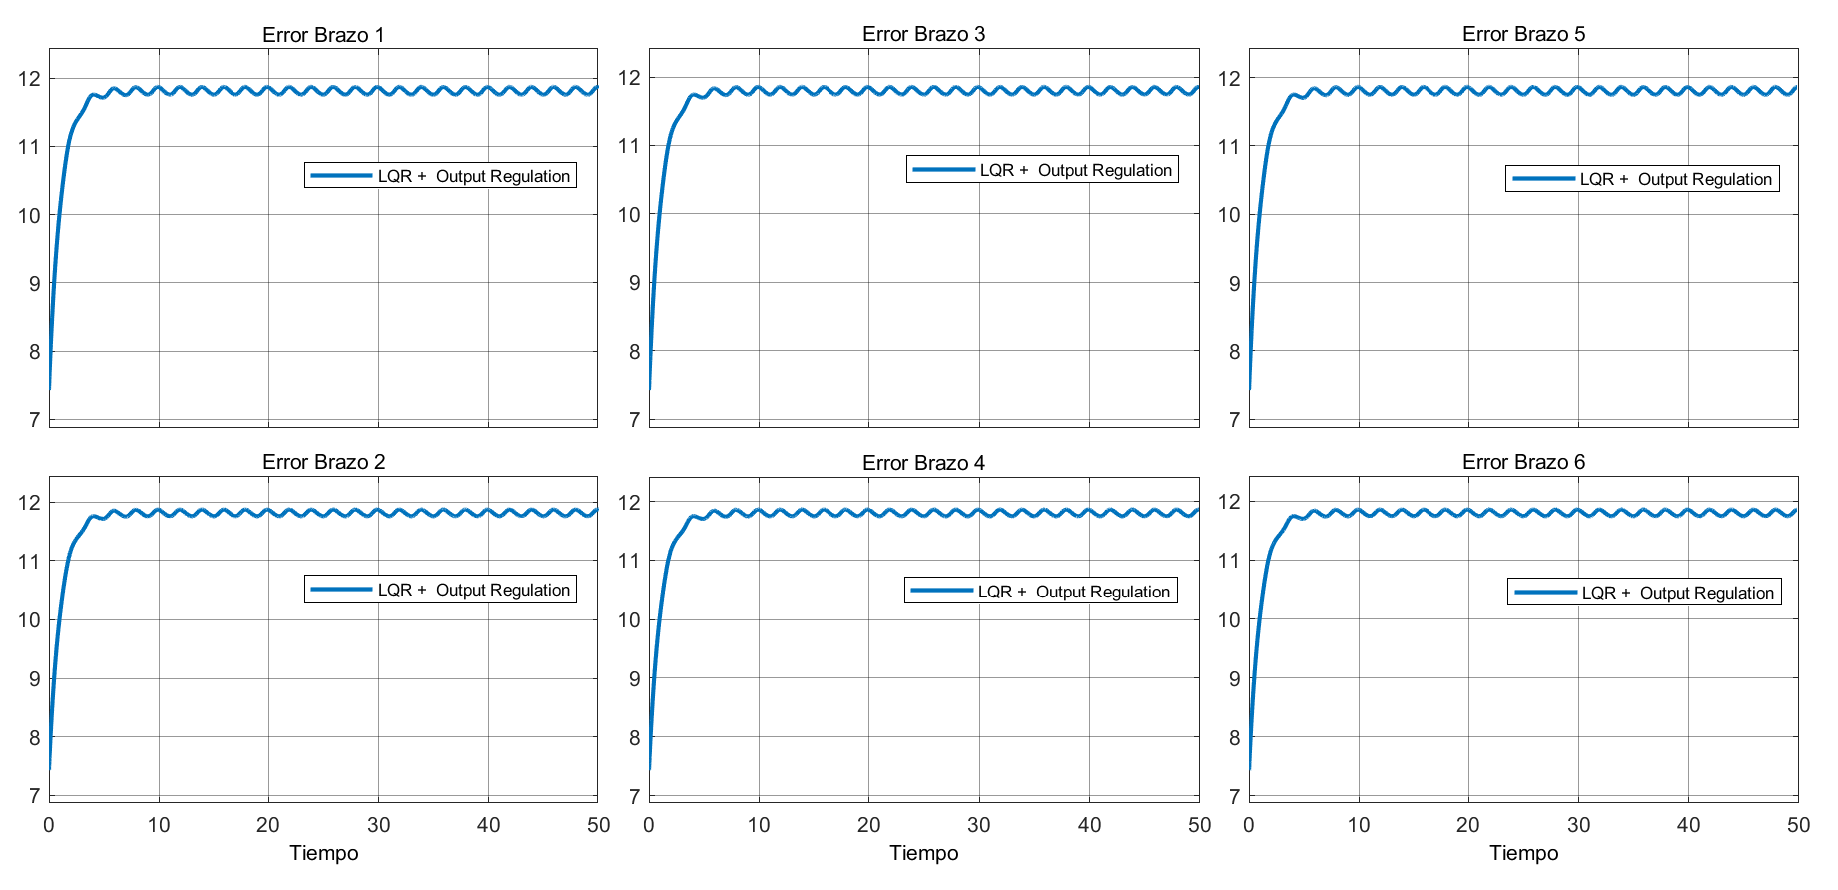
\includegraphics[width=0.9\columnwidth]{Results/lqrOR_frec_fija/lqr_sys_real_frec_fija.eps}
    \caption{Error de seguimiento (cm) LQR + Output Regulation sistema no-lineal, referencia frecuencia fija.}
    \label{fig:lqrOR_real_frec_fija}
\end{figure}

%--------------------------------------------------
\subsection{Referencia sinusoidal Nro.2 frecuencia, amplitud y fase variable}

Se define la referencia Nro.2 a seguir de cada brazo, con escalones y sinusoidales de distinta amplitud, frecuencia, y fase:
\begin{equation}
    l_{ref2}(t) = \begin{bmatrix}
        4 sin(0.5\pi t) + 8\\
        sin(\pi t) + 10\\
        sin(0.5\pi t) + 10\\
        sin(\pi t) + 10\\
        sin(0.5\pi t) + 10\\
        sin(\pi t) + 10\\
    \end{bmatrix}
\end{equation}

Se establecen así los parámetros de la referencia de amplitud, frecuencia y fase variable:
\begin{itemize}
    \item amplitud escalón $\Upsilon_{step1}=8$ y $\Upsilon_{step2}=\Upsilon_{step3}=\Upsilon_{step4}=\Upsilon_{step5}=\Upsilon_{step6}=10$.
    \item amplitud sinusoidal $\Upsilon_{sin1}=4$ y $\Upsilon_{sin2}=\Upsilon_{sin3}=\Upsilon_{sin4}=\Upsilon_{sin5}=\Upsilon_{sin6}=1$,\\ 
    frecuencia $\theta_1=\theta_3=\theta_5=0.5\pi$ y $\theta_2=\theta_4=\theta_6=\pi$, \\
    fase $\phi_1=\phi_2=\phi_3=\phi_4=\phi_5=\phi_6=0$.
\end{itemize}
 

Con los parámetros obtenidos de la referencia se modela su sistema exógeno de \ref{eq:sys_ref_variable}. Con el sistema exógeno de la referencia y los parámetros del sistema \ref{eq:sysStewart_outputregulation} de la plataforma Stewart, se obtiene la matriz feedforward $K_v$ del control para la referencia sinusoidal Nro.2:

\begin{multline}
    K_v = \scalebox{0.75}{$\left[ \begin{matrix}
        59.103 &	28.233 &	15.377 &	\textrm{-}29.820 &	\textrm{-}2.125 &	\textrm{-}0.547 &	\textrm{-}10.957 &	\textrm{-}1.023 &	\textrm{-}0.281 &	20.854 &	1.634 &	0.394 \\
        \textrm{-}23.809 &	\textrm{-}11.047 &	\textrm{-}2.181 &	73.682 &	6.050 &	3.842 &	\textrm{-}17.338 &	\textrm{-}1.749 &	\textrm{-}0.088 &	\textrm{-}4.819 &	\textrm{-}0.192 & \textrm{-}0.118 \\
        \textrm{-}3.875 &	\textrm{-}1.648 &	\textrm{-}0.475 &	\textrm{-}17.338 &	\textrm{-}1.793 &	\textrm{-}0.088 &	73.946 &	7.065 &	3.845 &	\textrm{-}29.876 &	\textrm{-}2.130 &	\textrm{-}0.547 \\
        16.725 &	7.911 &	1.582 &	\textrm{-}11.006 &	\textrm{-}0.811 &	\textrm{-}0.282 &	\textrm{-}29.907 &	\textrm{-}2.776 &	\textrm{-}0.548 &	74.108 &	6.092 &	3.846 \\
        \textrm{-}8.941 &	\textrm{-}4.181 &	\textrm{-}1.134 &	20.881 &	1.636 &	0.396 &	\textrm{-}4.822 &	\textrm{-}0.410 &	\textrm{-}0.118 &	\textrm{-}17.541 &	\textrm{-}1.813 &	\textrm{-}0.089 \\
        \textrm{-}13.878 &	\textrm{-}6.998 &	\textrm{-}0.353 &	\textrm{-}4.740 &	\textrm{-}0.184 &	\textrm{-}0.118 &	20.868 &	1.974 &	0.395 &	\textrm{-}11.063 &	\textrm{-}0.816 &	\textrm{-}0.282 \\
    \end{matrix} \right.$} \\
    \scalebox{0.75}{$\left. \begin{matrix}
        \textrm{-}4.997 &	\textrm{-}0.427 &	\textrm{-}0.120 &	\textrm{-}17.298 &	\textrm{-}1.789 &	\textrm{-}0.087 \\
        20.750 &	1.962 &	0.393 &	\textrm{-}10.849 &	\textrm{-}0.795 &	\textrm{-}0.280 \\
        \textrm{-}10.985 &	\textrm{-}1.026 &	\textrm{-}0.281 &	20.859 &	1.634 &	0.395 \\
        \textrm{-}17.514 &	\textrm{-}1.766 &	\textrm{-}0.089 &	\textrm{-}4.902 &	\textrm{-}0.200 &	\textrm{-}0.119 \\
        74.255 &	7.096 &	3.847 &	\textrm{-}29.912 &	\textrm{-}2.134 &	\textrm{-}0.548 \\
        \textrm{-}29.848 &	\textrm{-}2.770 &	\textrm{-}0.547 &	73.887 &	6.070 &	3.845 \\
    \end{matrix} \right]$}
\end{multline}


\subsubsection{Simulación Sistema Lineal}

En la Figura \ref{fig:lqrOR_lineal_frec_variable} se puede apreciar el error de seguimiento de los brazos actuadores del sistema lineal. Como se puede notar, el efecto del Output Regulation funciona perfectamente al seguir a la referencia sinusoidal de amplitud, frecuencia y fase variable, mostrando un error cero en estado estacionario para el sistema linealizado.
\begin{figure}[H]
\centering
    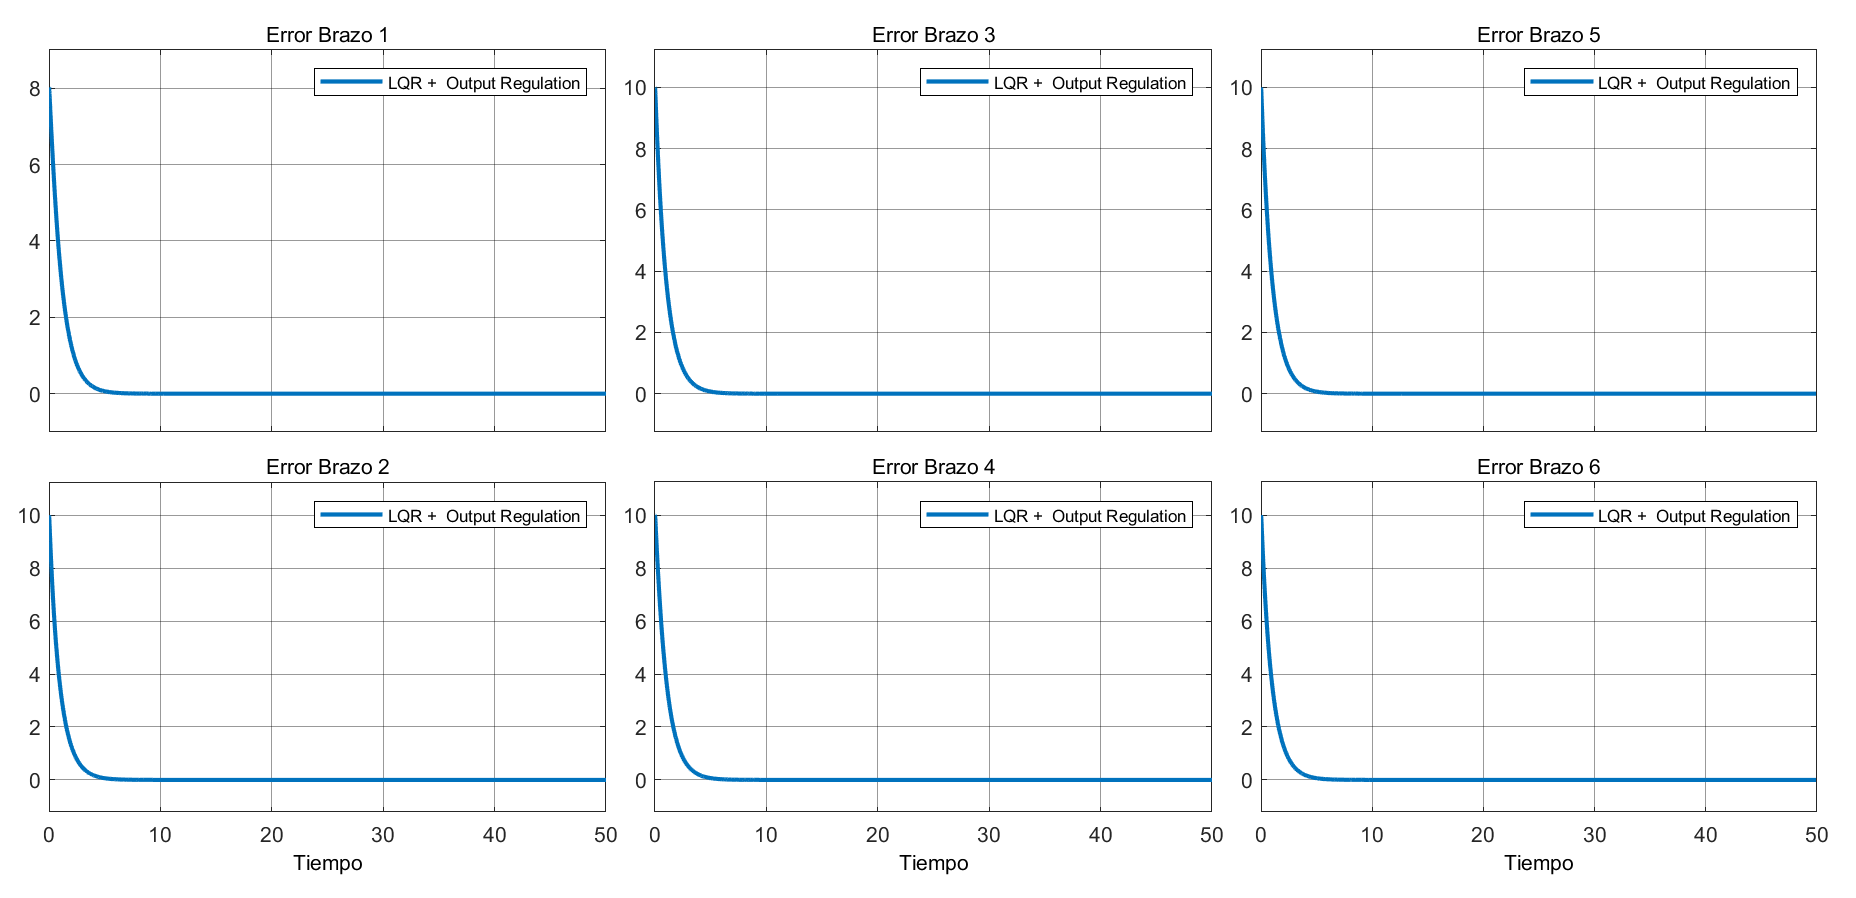
\includegraphics[width=0.87\columnwidth]{Results/lqrOR_frec_variable/lqr_sys_lineal_frec_variable.eps}
    \caption{Error de seguimiento (cm) LQR + Output Regulation sistema lineal, referencia frecuencia variable.}
    \label{fig:lqrOR_lineal_frec_variable}
\end{figure}

\subsubsection{Simulación Sistema No-Lineal}

Se utiliza el sistema no-lineal de la plataforma Stewart para la simulación, ilustrando los errores de seguimiento de los brazos en la Figura \ref{fig:lqrOR_real_frec_variable}.

Como se puede notar, se obtiene un error considerable en todos los brazos actuadores. Cada gráfica posee un valor de error constante junto a oscilaciones que se diferencian entre si. 
Por mucho que la nueva referencia sinusoidal de frecuencia variable haya sido incluida en el problema de Output Regulation, no fue suficiente para garantizar un seguimiento adecuado de esta referencia, es decir, error estacionario cero.

\begin{figure}[H]
\centering
    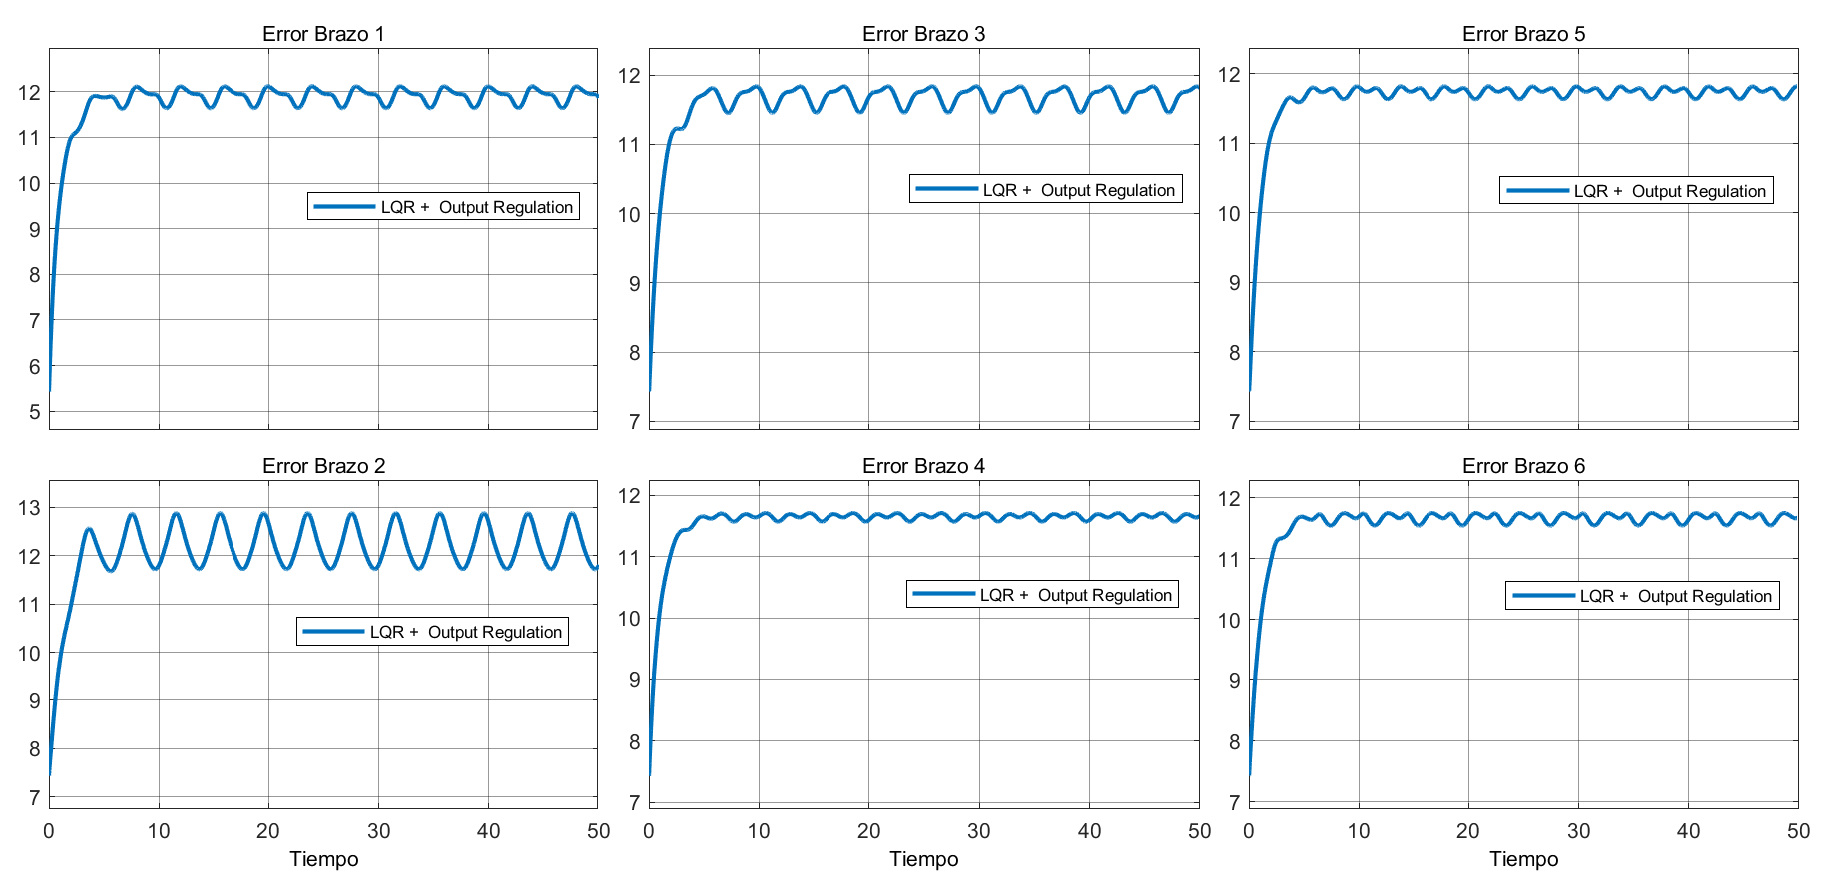
\includegraphics[width=0.87\columnwidth]{Results/lqrOR_frec_variable/lqr_sys_real_frec_variable.eps}
    \caption{Error de seguimiento (cm) LQR + Output Regulation sistema no-lineal, referencia frecuencia variable.}
    \label{fig:lqrOR_real_frec_variable}
\end{figure}


Con los resultados obtenidos en ambos casos de las referencias sinusoidal Nro.1 y Nro.2 (frecuencia fija y variable), podemos concluir que no es suficiente un controlador LQR con Output Regulation para el seguimiento sinusoidal. Las simulaciones con las plantas lineales dieron buenos resultados, pero al momento de modelar con el sistema no-lineal los resultados no eran los esperados. En primer lugar, se obtuvo un valor constante presente en todas las gráficas de error. En segundo lugar, un factor oscilante se presento también en todos estos errores. Tanto el valor constante como el oscilante, deben tratar de ser erradicados para lograr un control eficiente. 

Para lograr corregir los 2 defectos anteriores, se propone a continuación 2 ajustes al diseño de control desarrollado para el seguimiento a referencia sinusoidal. 




%###############################################
%###############################################
%###############################################
 \section{Diseño control LQI con Output Regulation posición velocidad}
\lhead[\thepage]{Sección \thesection. LQI con Output Regulation}

Se proponen 2 ajustes al control anterior para mejorar el desempeño y corregir los errores obtenidos:
\begin{itemize}
    \item \textbf{\underline{Control LQI:}} Adición de la integral del error como estado extra al sistema, para garantizar error de posición cero en estado estacionario para la componente constante de la referencia. Con esto se eliminará cualquier tipo de constante otorgada por parte de la referencia o de perturbaciones en el caso de que el sistema posea.

    \item \textbf{\underline{Output Regulation con posición y velocidad:}} Como la medición de la velocidad de los brazos actuadores esta disponible, se puede utilizar junto a la posición y velocidad de la referencia ya conocida, para aumentar la precisión en la regulación empleada para el seguimiento sinusoidal. De esta forma, se podrá disminuir aun más el error de seguimiento de la componente sinusoidal.
\end{itemize}

Se agrega la integral del error como estado extra, teniendo un estado aumentado al igual como se desarrolló en la sección \ref{sec:lqi_stewart} del capítulo \ref{cap:mimoPID}. Con el sistema aumentado LQI \ref{eq:sys_aumentado_lqi} y el sistema lineal \ref{eq:sysStewart_outputregulation} de la plataforma Stewart se tiene:

\begin{equation} 
    \begin{bmatrix}
        \dot{\xi}(t) \\ \dot{\xi}_{int}(t)
    \end{bmatrix} = \underbrace{\begin{bmatrix}
        A_0 & 0 \\ -C_0 & 0 
    \end{bmatrix}}_{A_a} \begin{bmatrix}
        \xi(t) \\ \xi_{int}(t)
    \end{bmatrix} + \underbrace{\begin{bmatrix}
        B_0 \\ 0
    \end{bmatrix}}_{B_a} u(t)
\end{equation}
donde $\xi_{int}(t) = \int e(t) dt= \int (r(t)-y(t)) dt = \int (r(t)-C_0 \xi(t)) dt$ es la integral del error de seguimiento de posición, y el nuevo estado aumentado definido como $z(t) = \begin{bmatrix} \xi(t)^\top & \xi_{int}(t)^\top\end{bmatrix}^\top$.

Resolviendo para la ley de control LQI como se desarrolla en la sección \ref{sec:lqicontrol} del capítulo \ref{cap:Notación y preliminares}, se obtienen las matrices de realimentación $K_\xi$ y $K_{int}$:
\begin{equation}
    u(t) = -K_\xi \xi(t) - K_{int} \xi_{int}(t)
\end{equation}

Posteriormente, se define la referencia incluyendo la velocidad como la derivada de la posición:
\begin{equation}
    \begin{bmatrix}
        l_{ref}(t) \\ \dot{l}_{ref}(t)
    \end{bmatrix} = \begin{bmatrix}
        \Upsilon_{pos1} sin(\theta_1 t + \phi_1) + \Upsilon_{step1}\\
        \Upsilon_{pos2} sin(\theta_2 t + \phi_2) + \Upsilon_{step2}\\
        \Upsilon_{pos3} sin(\theta_3 t + \phi_3) + \Upsilon_{step3}\\
        \Upsilon_{pos4} sin(\theta_4 t + \phi_4) + \Upsilon_{step4}\\
        \Upsilon_{pos5} sin(\theta_5 t + \phi_5) + \Upsilon_{step5}\\
        \Upsilon_{pos6} sin(\theta_6 t + \phi_6) + \Upsilon_{step6}\\
        \Upsilon_{pos1} \theta_1 cos(\theta_1 t + \phi_1)\\
        \Upsilon_{pos2} \theta_2 cos(\theta_2 t + \phi_2)\\
        \Upsilon_{pos3} \theta_3 cos(\theta_3 t + \phi_3)\\
        \Upsilon_{pos4} \theta_4 cos(\theta_4 t + \phi_4)\\
        \Upsilon_{pos5} \theta_5 cos(\theta_5 t + \phi_5)\\
        \Upsilon_{pos6} \theta_6 cos(\theta_6 t + \phi_6)\\
    \end{bmatrix}
\end{equation}

Se modela la referencia como sistema exógeno de la forma:
\begin{align} \label{eq:ref_exogeno_LQI_OR}
    \dot{v}(t) & = H_v v(t), \notag \\
    \begin{bmatrix}
        l_{ref}(t) \\ \dot{l}_{ref}(t)
    \end{bmatrix} & = C_v v(t)
\end{align}
donde 
\begin{gather}
    H_v = \begin{bmatrix}
        H_{v1} & \hdots & 0 \\
        \vdots & \ddots & \vdots \\ 
        0 & \hdots & H_{v6}
    \end{bmatrix}, 
    \quad \textrm{con } \quad
    H_{vi} = \begin{bmatrix}
        0 & 0 & 0 \\
        0 & 0 & 1 \\
        0 & -\theta_i^2 & 0
    \end{bmatrix},  \\
    C_v = \begin{bmatrix}
        C_{v1\_pos} & \hdots & 0 \\
        \vdots & \ddots & \vdots \\ 
        0 & \hdots & C_{v6\_pos} \\
        C_{v1\_vel} & \hdots & 0 \\
        \vdots & \ddots & \vdots \\ 
        0 & \hdots & C_{v6\_vel}
    \end{bmatrix}, \notag \\
    \quad \textrm{con } \quad
    C_{vi\_pos} = \begin{bmatrix}
        \Upsilon_{step\textrm{ }i} & \Upsilon_{pos\textrm{ }i} & 0
    \end{bmatrix},
    \quad 
    C_{vi\_vel} = \begin{bmatrix}
        0 & 0 & \theta_i \Upsilon_{pos\textrm{ }i}
    \end{bmatrix}, \\
    v(0) = \begin{bmatrix}
        \begin{bmatrix} 1 & sin(\phi_1) & cos(\phi_1) \end{bmatrix} & \hdots & \begin{bmatrix} 1 & sin(\phi_6) & cos(\phi_6) \end{bmatrix} 
    \end{bmatrix}, \quad
    \textrm{tal que } i = 1,\hdots,6 \notag
\end{gather}

Con la nueva referencia con velocidad incluida y la nueva matriz de los estados internos del sistema $(-K_\xi)$ (se incluye signo negativo), se resuelven las ecuaciones de regulación para $X$ y $U$ (demostrado en Apéndice \ref{appen1}) en el problema de Output Regulation de posición y velocidad:

\begin{align}
    X H_v = A_0 X + B_0 U \notag \\
    0 = C_0 X + D_0 U - C_v 
\end{align}

Con $A_0, B_0, C_0, D_0$ las matrices del sistema lineal \ref{eq:sysStewart_outputregulation} de la plataforma Stewart, donde $C_0$ nos permite medir directamente posición y velocidad de los brazos. Además $C_v$ corresponde a la referencia deseada de la posición y de la velocidad de los brazos.

Con $X$ y $U$ obtenidos se despeja $K_v$ desde la igualdad $K_v = U - (-K_\xi) X$.

Finalmente, se obtiene la ley de control LQI con Output Regulation posición velocidad para referencias sinusoidales de la forma:

\begin{equation}
    u(t) = -K_\xi \xi(t) - K_{int} \xi_{int}(t) + K_v v(t)
\end{equation}
con $\xi(t)$ los estados de la plataforma Stewart (posición y velocidad de brazos), $\xi_{int}(t)$ el estado de la integral del error de posición y $v(t)$ el estado interno del sistema exógeno de la referencia.

En la Figura \ref{fig:lqi_OR_stewart_scheme} se puede ilustrar el nuevo esquema de control LQI con Output Regulation posición velocidad. 

\begin{figure}[ht]
\centering
    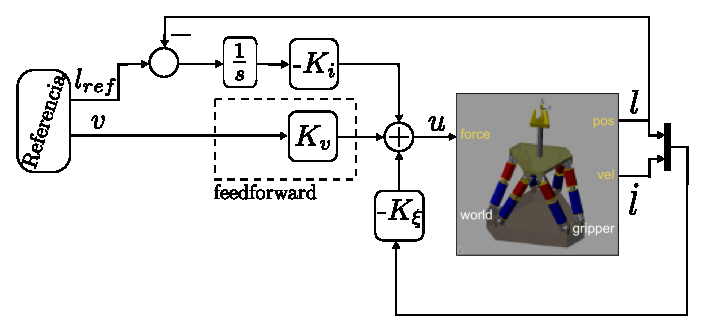
\includegraphics[width=0.8\columnwidth]{Figures/Output_Regulation/lqi_OR_stewart_scheme.eps}
    \caption{Esquema de control LQI con Output Regulation posición velocidad para la plataforma Stewart.}
    \label{fig:lqi_OR_stewart_scheme}
\end{figure}

 \section{Resultados de simulación control LQI con Output Regulation posición velocidad}
\lhead[\thepage]{Sección \thesection. Resultados de simulación control LQI con Output Regulation}

Los resultados de simulación del control LQI con Output Regulation posición velocidad para seguimiento sinusoidal, se compararán con el controlador de mejor desempeño del capítulo \ref{cap:mimoPID} anterior. Recordando, el controlador MIMO PID Full del capítulo \ref{cap:mimoPID} demostraba tener un mejor seguimiento de la referencia, así como mejores índices de desempeño en comparación con sus versiones descentralizadas. El principal problema que presenta es en el seguimiento de referencia sinusoidal, ya que la magnitud del error de seguimiento es significativo.

\begin{remark}
Las matrices $K_P$, $K_D$ y $K_I$ del controlador MIMO PID Full utilizadas son las mismas mostradas en \ref{eq:KP_mimoPID}, \ref{eq:KD_mimoPID} y \ref{eq:KI_mimoPID}, en los resultados del Caso 2 de la sección \ref{sec:resultados_mimoPID} del capítulo \ref{cap:mimoPID}.
\end{remark}

Se utilizan las matrices $A_0, B_0, C_0, D_0$ del sistema lineal \ref{eq:sysStewart_outputregulation} de la plataforma Stewart.

Para el diseño del control LQI con Output Regulation, se utilizan las siguientes matrices $Q$ y $R$ para la obtención de las matrices de realimentación:
\begin{equation}
    Q = \begin{bmatrix} C_0^\top C_0 & 0 \\ 0 & 100\cdot I_{6\times6} \end{bmatrix}, \qquad R = 0.1\cdot I_{6\times6} 
\end{equation}
La explicación del $Q$ anterior es la misma mencionada en el capítulo \ref{cap:mimoPID}, es decir, se ponderan los estados correspondientes a la integral del error por sobre los demás para así darle más importancia al seguimiento de la referencia. Por otro lado, la matriz $R$ utilizada es de baja ponderación para la señal de actuación, para así no restringir demasiado su efecto en el sistema.

Con $Q$ y $R$ dados, las matrices de realimentación $K_\xi$ y $K_{int}$ para el control LQI con Output Regulation posición velocidad son:

\begin{equation}
    K_\xi = \scalebox{0.8}{$\begin{bmatrix}
        24.037 &	\textrm{-}6.357 &	\textrm{-}2.141 &	3.812 &	\textrm{-}1.493 &	\textrm{-}2.746 & 4.150 &	\textrm{-}0.710 &	\textrm{-}0.304 &	0.443 &	\textrm{-}0.194 &	\textrm{-}0.038 \\
        \textrm{-}6.363 &	24.013 &	\textrm{-}2.739 &	\textrm{-}1.479 &	3.807 &	\textrm{-}2.125 & \textrm{-}0.709 &	4.148 &	\textrm{-}0.038 &	\textrm{-}0.193 &	0.442 &	\textrm{-}0.303 \\
        \textrm{-}1.478 &	\textrm{-}2.785 &	24.078 &	\textrm{-}6.361 &	\textrm{-}2.137 &	3.807 & \textrm{-}0.193 &	\textrm{-}0.038 &	4.158 &	\textrm{-}0.710 &	\textrm{-}0.304 &	0.443 \\
        3.784 &	\textrm{-}2.159 &	\textrm{-}6.351 &	24.089 &	\textrm{-}2.786 &	\textrm{-}1.467 & 0.444 &	\textrm{-}0.305 &	\textrm{-}0.711 &	4.151 &	\textrm{-}0.039 &	\textrm{-}0.193 \\
        \textrm{-}2.181 &	3.768 &	\textrm{-}1.452 &	\textrm{-}2.777 &	24.093 &	\textrm{-}6.341 & \textrm{-}0.306 &	0.445 &	\textrm{-}0.192 &	\textrm{-}0.040 &	4.152 &	\textrm{-}0.711 \\
        \textrm{-}2.773 &	\textrm{-}1.461 &	3.799 &	\textrm{-}2.136 &	\textrm{-}6.370 &	24.065 & \textrm{-}0.039 &	\textrm{-}0.192 &	0.443 &	\textrm{-}0.304 &	\textrm{-}0.710 &	4.150 \\
    \end{bmatrix}$}
\end{equation}

\begin{equation}
    K_{int} = \begin{bmatrix}
    	\textrm{-}31.611 &	0.005 &	0.577 &	0.004 &	\textrm{-}0.594 &	\textrm{-}0.005 \\
    	\textrm{-}0.005 &	\textrm{-}31.611 &	\textrm{-}0.0002 &	\textrm{-}0.594 & 0.012 & 0.576 \\
    	\textrm{-}0.588 &	0.0006 &	\textrm{-}31.611 &	\textrm{-}0.002 &	0.582 &	0.0005 \\
    	\textrm{-}0.004 &	0.584 &	0.002 &	\textrm{-}31.611 &	\textrm{-}0.002 &	\textrm{-}0.592 \\
    	0.583 &	\textrm{-}0.012 &	\textrm{-}0.593 &	0.002 &	\textrm{-}31.611 &	0.005 \\
    	0.005 &	\textrm{-}0.587 &	\textrm{-}0.0008 &	0.581 &	\textrm{-}0.005 &	\textrm{-}31.611 \\
    \end{bmatrix}
\end{equation}

%--------------------------------------------------
\subsection{Referencia sinusoidal Nro.1 frecuencia fija}

Se establece la referencia sinusoidal Nro.1 de frecuencia fija, para el seguimiento de los brazos actuadores:

\begin{equation}
    \begin{bmatrix}
        l_{ref1}(t) \\ \dot{l}_{ref1}(t)
    \end{bmatrix} = \begin{bmatrix}
        2 sin(\pi t ) + 10\\
        2 sin(\pi t ) + 10\\
        2 sin(\pi t ) + 10\\
        2 sin(\pi t ) + 10\\
        2 sin(\pi t ) + 10\\
        2 sin(\pi t ) + 10\\
        2 \pi cos(\pi t )\\
        2 \pi cos(\pi t )\\
        2 \pi cos(\pi t )\\
        2 \pi cos(\pi t )\\
        2 \pi cos(\pi t )\\
        2 \pi cos(\pi t )\\
    \end{bmatrix}
\end{equation}

Se definen así los siguientes parámetros de la referencia:
\begin{itemize}
    \item amplitud escalón $\Upsilon_{step1}=\Upsilon_{step2}=\Upsilon_{step3}=\Upsilon_{step4}=\Upsilon_{step5}=\Upsilon_{step6}=10$.
    \item amplitud sinusoidal posición $\Upsilon_{pos1}=\Upsilon_{pos2}=\Upsilon_{pos3}=\Upsilon_{pos4}=\Upsilon_{pos5}=\Upsilon_{pos6}=2$, \\
    frecuencia $\theta_1=\theta_2=\theta_3=\theta_4=\theta_5=\theta_6=\pi$, \\
    fase $\phi_1=\phi_2=\phi_3=\phi_4=\phi_5=\phi_6=0$.
\end{itemize}

Con los parámetros obtenidos de la referencia se modela su sistema exógeno de \ref{eq:ref_exogeno_LQI_OR}. Con el sistema exógeno de la referencia y los parámetros del sistema \ref{eq:sysStewart_outputregulation} de la plataforma Stewart, se obtiene la matriz feedforward $K_v$ del control para la referencia sinusoidal Nro.1:

\begin{multline}
    K_v = \scalebox{0.75}{$\left[\begin{matrix}
        179.928 &  33.348 &  8.300 & \textrm{-}24.813 & \textrm{-}3.247 & \textrm{-}1.421 & \textrm{-}11.375 & \textrm{-}1.695  & \textrm{-}0.608 &  16.930 & 2.482 & 0.887 \\
      \textrm{-}24.745 &  \textrm{-}3.233 &  \textrm{-}1.419 & 179.818 &  33.326  &  8.297 &  \textrm{-}7.309  & \textrm{-}1.579  & \textrm{-}0.077 &  \textrm{-}4.416  & \textrm{-}0.303  & \textrm{-}0.386 \\
       \textrm{-}4.446 &  \textrm{-}0.309  & \textrm{-}0.387 &  \textrm{-}7.312 &  \textrm{-}1.580 &  \textrm{-}0.077 & 179.974 &  33.357  &  8.301 & \textrm{-}24.837 &  \textrm{-}3.252 &  \textrm{-}1.421 \\
       16.989  &  2.494 &   0.889 & \textrm{-}11.429 &  \textrm{-}1.706 &  \textrm{-}0.610 & \textrm{-}24.863 &  \textrm{-}3.257 &  \textrm{-}1.422 & 180.067 &  33.376  &  8.303 \\
      \textrm{-}11.511 &  \textrm{-}1.722 &  \textrm{-}0.612 &  16.997  &  2.495  &  0.890 &  \textrm{-}4.395 &  \textrm{-}0.299  & \textrm{-}0.385 &  \textrm{-}7.448  & \textrm{-}1.607 &  \textrm{-}0.080 \\
       \textrm{-}7.342 &  \textrm{-}1.586 &  \textrm{-}0.078 &  \textrm{-}4.388 &  \textrm{-}0.297 &  \textrm{-}0.385 &  16.937  &  2.483  &  0.887 & \textrm{-}11.422 &  \textrm{-}1.704 &  \textrm{-}0.609 
    \end{matrix}\right.$} \\
    \scalebox{0.75}{$\left. \begin{matrix}
        \textrm{-}4.508 &  \textrm{-}0.321 & \textrm{-}0.388 & \textrm{-}7.281 & \textrm{-}1.574 & \textrm{-}0.076 \\
        16.846  &  2.465 &   0.885 & \textrm{-}11.311 &  \textrm{-}1.682 & \textrm{-}0.606 \\
        \textrm{-}11.382 &  \textrm{-}1.696 &  \textrm{-}0.608 &  16.928 &   2.481 & 0.887 \\
        \textrm{-}7.418  & \textrm{-}1.601 &  \textrm{-}0.079 &  \textrm{-}4.438 &  \textrm{-}0.307 & \textrm{-}0.386 \\
        180.128 &  33.388 &   8.304 & \textrm{-}24.866 &  \textrm{-}3.258 & \textrm{-}1.422 \\
        \textrm{-}24.799  & \textrm{-}3.244 &  \textrm{-}1.420 & 179.937 &  33.350 & 8.300
    \end{matrix}\right]$}
\end{multline}

Para un tiempo de simulación de $T_{sim}=50(s)$ se obtienen las gráficas de error de posición y fuerza de actuación mostradas en las Figuras \ref{fig:lqiOR_error_frec_fija} y \ref{fig:lqiOR_fuerza_frec_fija} respectivamente. 
En primera instancia si comparamos el error del control LQI Output Regulation (Figura \ref{fig:lqiOR_error_frec_fija}) con el error del control LQR Output Regulation (Figura \ref{fig:lqrOR_real_frec_fija}), notamos una mejora considerable al utilizar el integrador del control LQI, ya que elimina el valor constante que presenta el error del control LQR. Por otro lado, es evidente que el control MIMO PID Full no es capaz de seguir correctamente a la referencia sinusoidal evidenciado en los altos valores del error de seguimiento que posee. Finalmente, al utilizar Output Regulation podemos notar que el error en cada brazo disminuye considerablemente con la matriz feedforward $K_v$ de la referencia. Esta matriz permite el seguimiento de la señal de manera más eficiente como se aprecia en la gráfica, logrando magnitudes del error muy pequeñas del orden de los $0.02$. 

Con respecto a las fuerzas aplicadas en los brazos actuadores (Figura \ref{fig:lqiOR_fuerza_frec_fija}), podemos notar que el controlador MIMO PID Full posee actuaciones más pequeñas que el control LQI con Output Regulation. Por mucho que la actuación sea levemente menor, el control MIMO PID Full no es suficiente para el seguimiento sinusoidal como se aprecia en la gráfica del error. La diferencia de actuación con el control LQI Output Regulation radica en que este está enfocado en seguir a la referencia sinusoidal de mejor manera, por ende, necesita de más actuación para el control.
\newpage
\begin{figure}[H]
\centering
    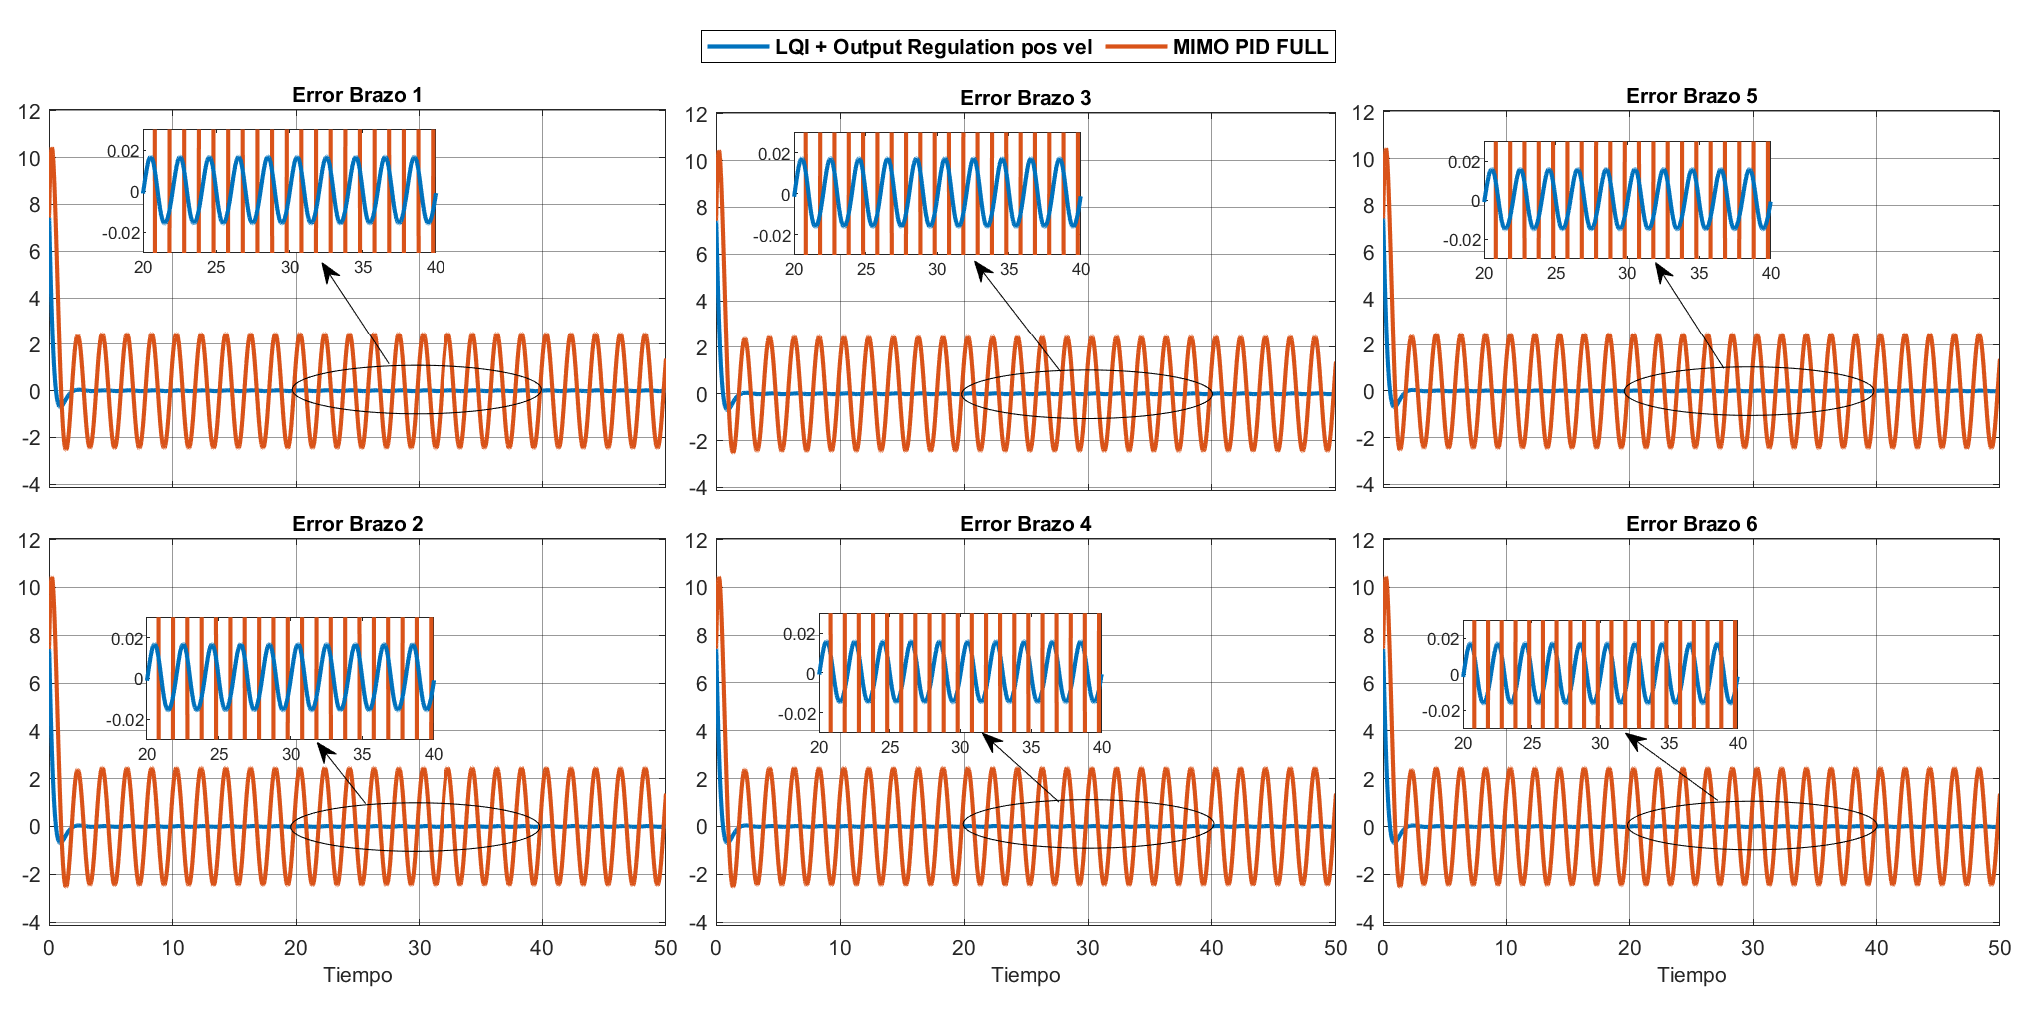
\includegraphics[width=1\columnwidth]{Results/LQI_OR_frec_fija/error_frec_fija.eps}
    \caption{Error de seguimiento (cm) LQI+OR v/s MIMO PID Full, referencia frecuencia fija.}
    \label{fig:lqiOR_error_frec_fija}
\end{figure}

\begin{figure}[H]
\centering
    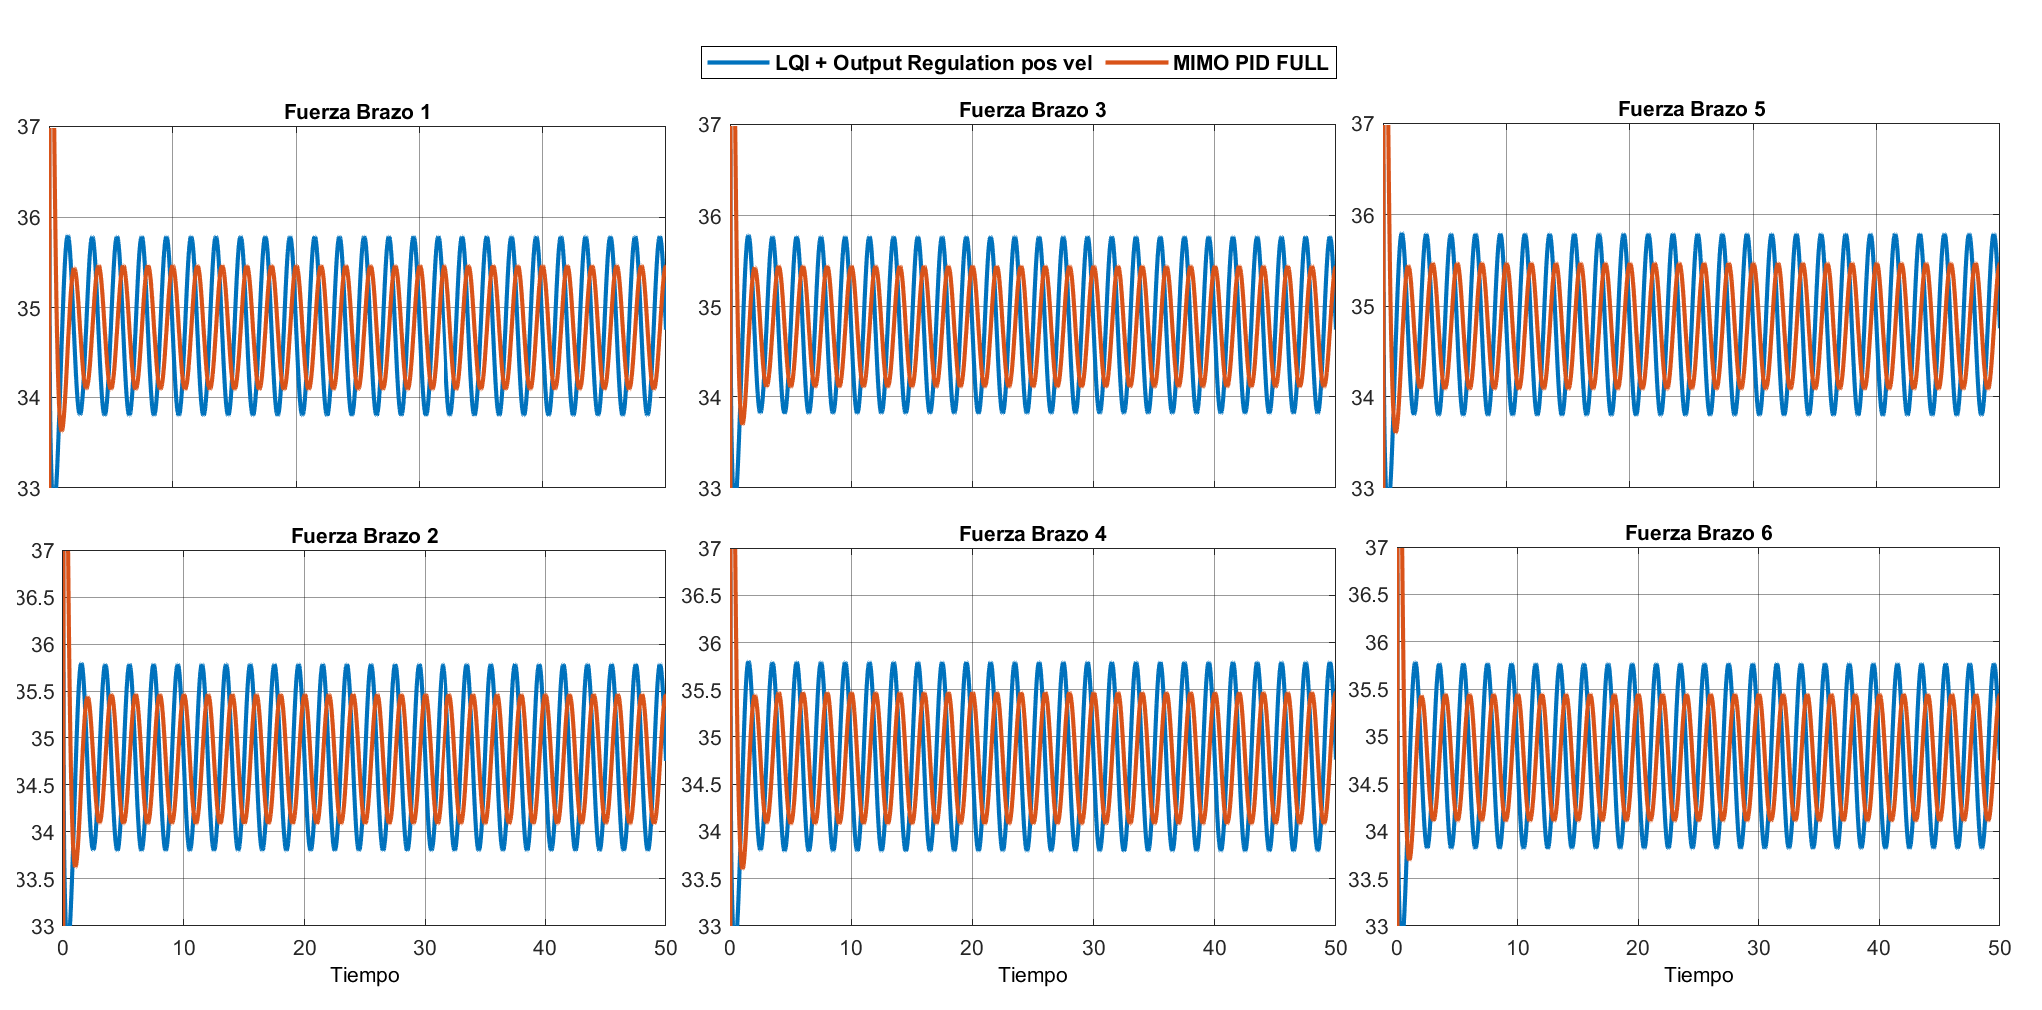
\includegraphics[width=1\columnwidth]{Results/LQI_OR_frec_fija/fuerza_frec_fija.eps}
    \caption{Fuerza de actuación (N) LQI+OR v/s MIMO PID Full, referencia frecuencia fija.}
    \label{fig:lqiOR_fuerza_frec_fija}
\end{figure}

\newpage
%--------------------------------------------------
\subsection{Referencia sinusoidal Nro.2 frecuencia, amplitud y fase variable}

Se establece la referencia sinusoidal Nro.2 de frecuencia, amplitud y fase variable, para el seguimiento de los brazos actuadores:

\begin{equation}
    \begin{bmatrix}
        l_{ref2}(t) \\ \dot{l}_{ref2}(t)
    \end{bmatrix} = \begin{bmatrix}
        4 sin(0.5\pi t ) + 8\\
        sin(\pi t ) + 10\\
        sin(0.5\pi t ) + 10\\
        sin(\pi t ) + 10\\
        sin(0.5\pi t ) + 10\\
        sin(\pi t ) + 10\\
        4(0.5\pi) cos(0.5\pi t )\\
        \pi cos(\pi t )\\
        0.5\pi cos(0.5\pi t )\\
        \pi cos(\pi t )\\
        0.5\pi cos(0.5\pi t )\\
        \pi cos(\pi t )\\
    \end{bmatrix}
\end{equation}

Se definen así los siguientes parámetros:
\begin{itemize}
    \item amplitud escalón $\Upsilon_{step1}=8$ y $\Upsilon_{step2}=\Upsilon_{step3}=\Upsilon_{step4}=\Upsilon_{step5}=\Upsilon_{step6}=10$.
    \item amplitud sinusoidal posición $\Upsilon_{pos1}=4$ y $\Upsilon_{pos2}=\Upsilon_{pos3}=\Upsilon_{pos4}=\Upsilon_{pos5}=\Upsilon_{pos6}=1$, \\
    frecuencia $\theta_1=\theta_3=\theta_5=0.5\pi$ y $\theta_2=\theta_4=\theta_6=\pi$, \\
    fase $\phi_1=\phi_2=\phi_3=\phi_4=\phi_5=\phi_6=0$.
\end{itemize}

Con los parámetros obtenidos de la referencia se modela su sistema exógeno de \ref{eq:ref_exogeno_LQI_OR}. Con el sistema exógeno de la referencia y los parámetros del sistema \ref{eq:sysStewart_outputregulation} de la plataforma Stewart, se obtiene la matriz feedforward $K_v$ del control para la referencia sinusoidal Nro.2:

\begin{multline}
    K_v = \scalebox{0.75}{$\left[\begin{matrix}
        143.943	& 70.653 &	16.601 &	\textrm{-}24.813	& \textrm{-}1.624 &	\textrm{-}0.711 &	\textrm{-}11.375	& \textrm{-}1.065 &	\textrm{-}0.304 & 	16.931 &	1.241 &	0.444  \\
        \textrm{-}19.796 &	\textrm{-}9.041 &	\textrm{-}2.838 &	179.818 &	16.663 &	4.149 &	\textrm{-}7.309 &	\textrm{-}0.746 &	\textrm{-}0.039 &	\textrm{-}4.417 &	\textrm{-}0.152 &	\textrm{-}0.193  \\
        \textrm{-}3.557 &	\textrm{-}1.489 &	\textrm{-}0.775 &	\textrm{-}7.313 &	\textrm{-}0.790 &	\textrm{-}0.039 &	179.974 &	17.668 &	4.151 &	\textrm{-}24.837 &	\textrm{-}1.626 &	\textrm{-}0.711 \\
        13.591 &	6.344 &	1.779 &	\textrm{-}11.430 &	\textrm{-}0.853 &	\textrm{-}0.305 &	\textrm{-}24.864	& \textrm{-}2.272 &	\textrm{-}0.711 &	180.068 &	16.688 &	4.152 \\
        \textrm{-}9.209 &	\textrm{-}4.315 &	\textrm{-}1.224 &	16.998 &	1.248 &	0.445 &	\textrm{-}4.395 &	\textrm{-}0.367 &	\textrm{-}0.193 &	\textrm{-}7.449 &	\textrm{-}0.804 &	\textrm{-}0.040  \\
        \textrm{-}5.874 &	\textrm{-}2.996 &	\textrm{-}0.157 &	\textrm{-}4.388 &	\textrm{-}0.149 &	\textrm{-}0.193 &	16.937 &	1.581 &	0.444 &	\textrm{-}11.423 &	\textrm{-}0.852 &	\textrm{-}0.305	\\
    \end{matrix}\right.$} \\
    \scalebox{0.75}{$\left.\begin{matrix}
        \textrm{-}4.508 &	\textrm{-}0.378 &	\textrm{-}0.195 &	\textrm{-}7.282 &	\textrm{-}0.787 &	\textrm{-}0.038 \\
        16.847 &	1.572 &	0.443 &	\textrm{-}11.311	& \textrm{-}0.841 &	\textrm{-}0.303 \\
        \textrm{-}11.382 &	\textrm{-}1.066 &	\textrm{-}0.304 &	16.929 &	1.241 &	0.444 \\
        \textrm{-}7.418 &	\textrm{-}0.757 &	\textrm{-}0.040 &	\textrm{-}4.439 &	\textrm{-}0.154 &	\textrm{-}0.193 \\
        180.129 &	17.683 &	4.152 &	\textrm{-}24.867 &	\textrm{-}1.629 &	\textrm{-}0.711 \\
        \textrm{-}24.799 &	\textrm{-}2.266 &	\textrm{-}0.710 &	179.937 &	16.675 &	4.150 \\
    \end{matrix}\right]$}
\end{multline}

Para un tiempo de simulación de $T_{sim}=50(s)$ se obtienen las gráficas de error de posición y fuerza de actuación mostradas en las Figuras \ref{fig:lqiOR_error_frec_variable} y \ref{fig:lqiOR_fuerza_frec_variable} respectivamente. En primera instancia, al comparar el error del control LQI Output Regulation (Figura \ref{fig:lqiOR_error_frec_variable}) con el error del control LQR Output Regulation (Figura \ref{fig:lqrOR_real_frec_variable}) podemos ver que el integrador utilizado en el control LQI logra eliminar completamente la constante presente en todos los errores del control LQR. Por otro lado, en comparación con el control MIMO PID Full se puede notar claramente que el efecto del Output Regulation logra disminuir considerablemente el error de seguimiento en cada brazo, pasando de magnitudes cercanas de $3$ y $1$ para el control MIMO PID Full, a magnitudes cercanas de $0.4$ y $0.1$ respectivamente para el control LQI Output Regulation.

Por otro lado en la Figura \ref{fig:lqiOR_fuerza_frec_variable} , las fuerzas actuadoras del control LQI Output Regulation son levemente mayores que el control MIMO PID Full, ya que posee un objetivo extra que es el seguimiento sinusoidal a diferencia del control MIMO PID Full.

\begin{figure}[H]
\centering
    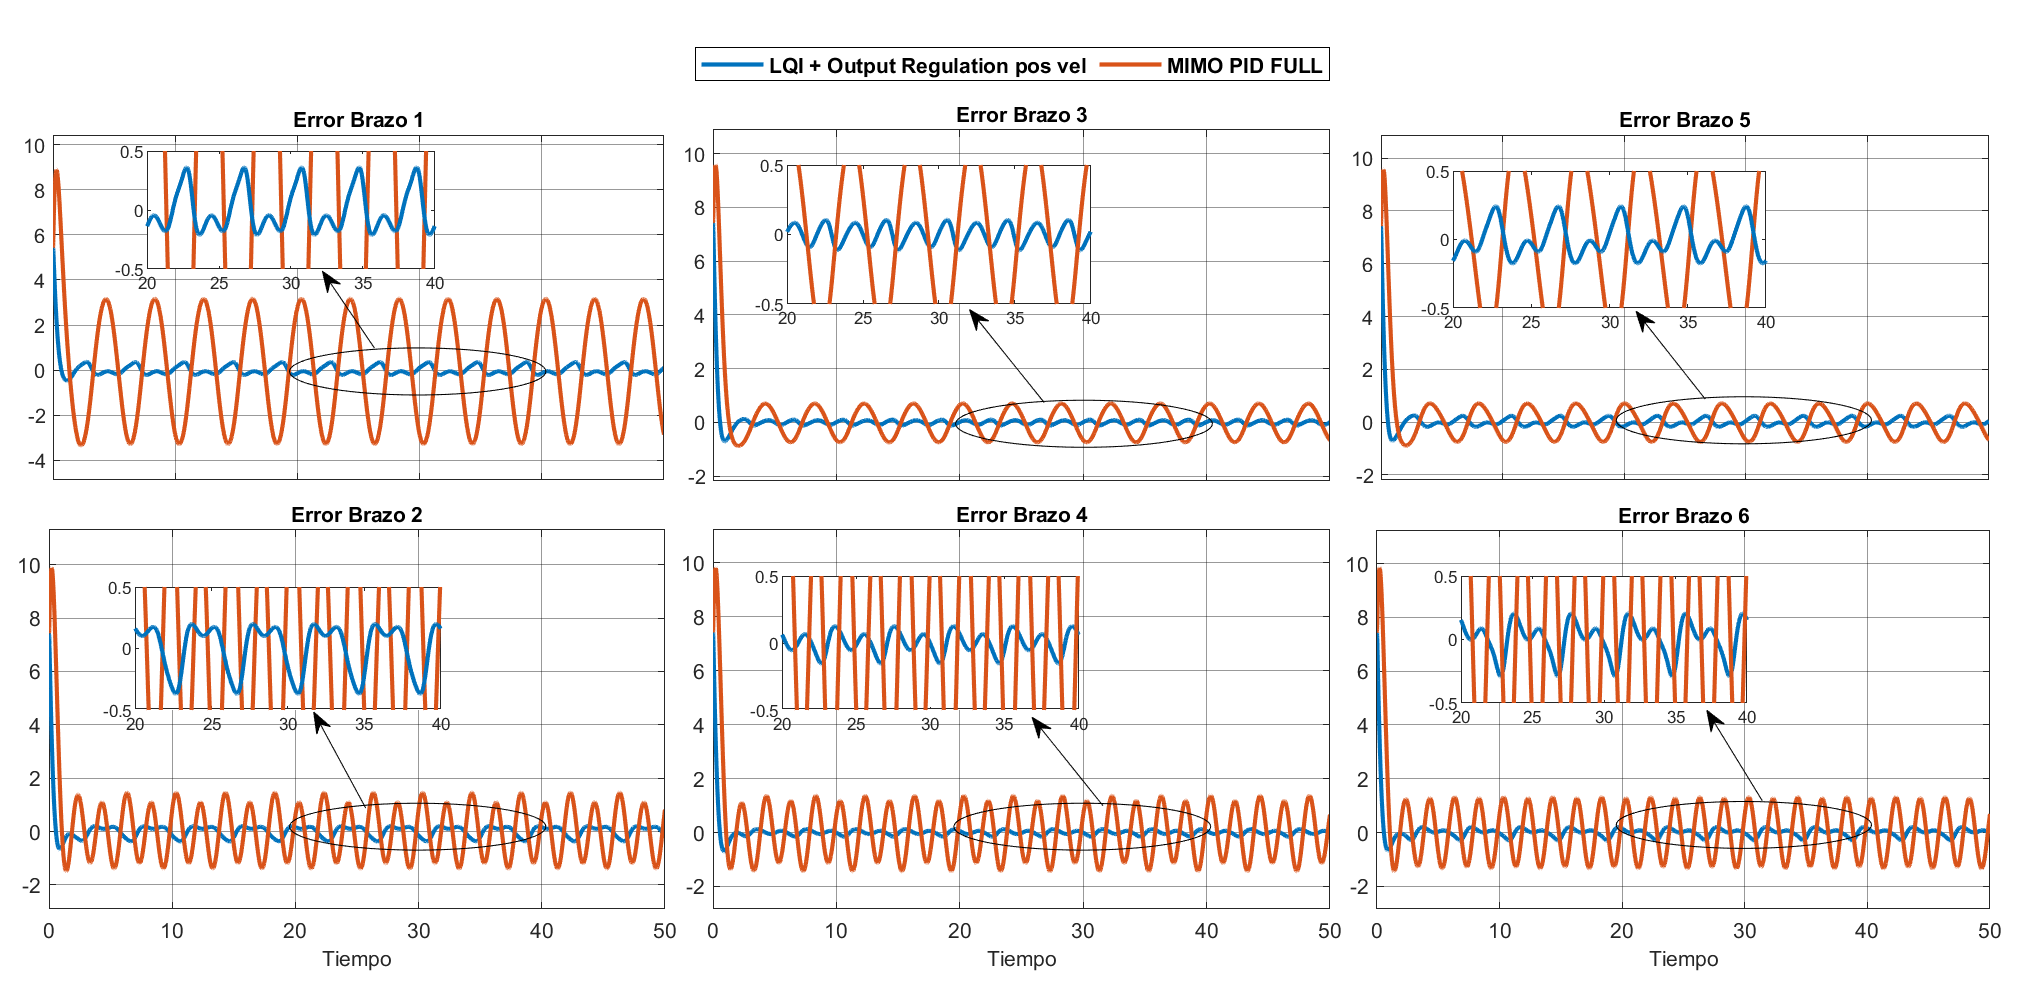
\includegraphics[width=1\columnwidth]{Results/LQI_OR_frec_variable/error_frec_variable.eps}
    \caption{Error de seguimiento (cm) LQI+OR v/s MIMO PID Full, referencia frecuencia variable.}
    \label{fig:lqiOR_error_frec_variable}
\end{figure}
\newpage
\begin{figure}[H]
\centering
    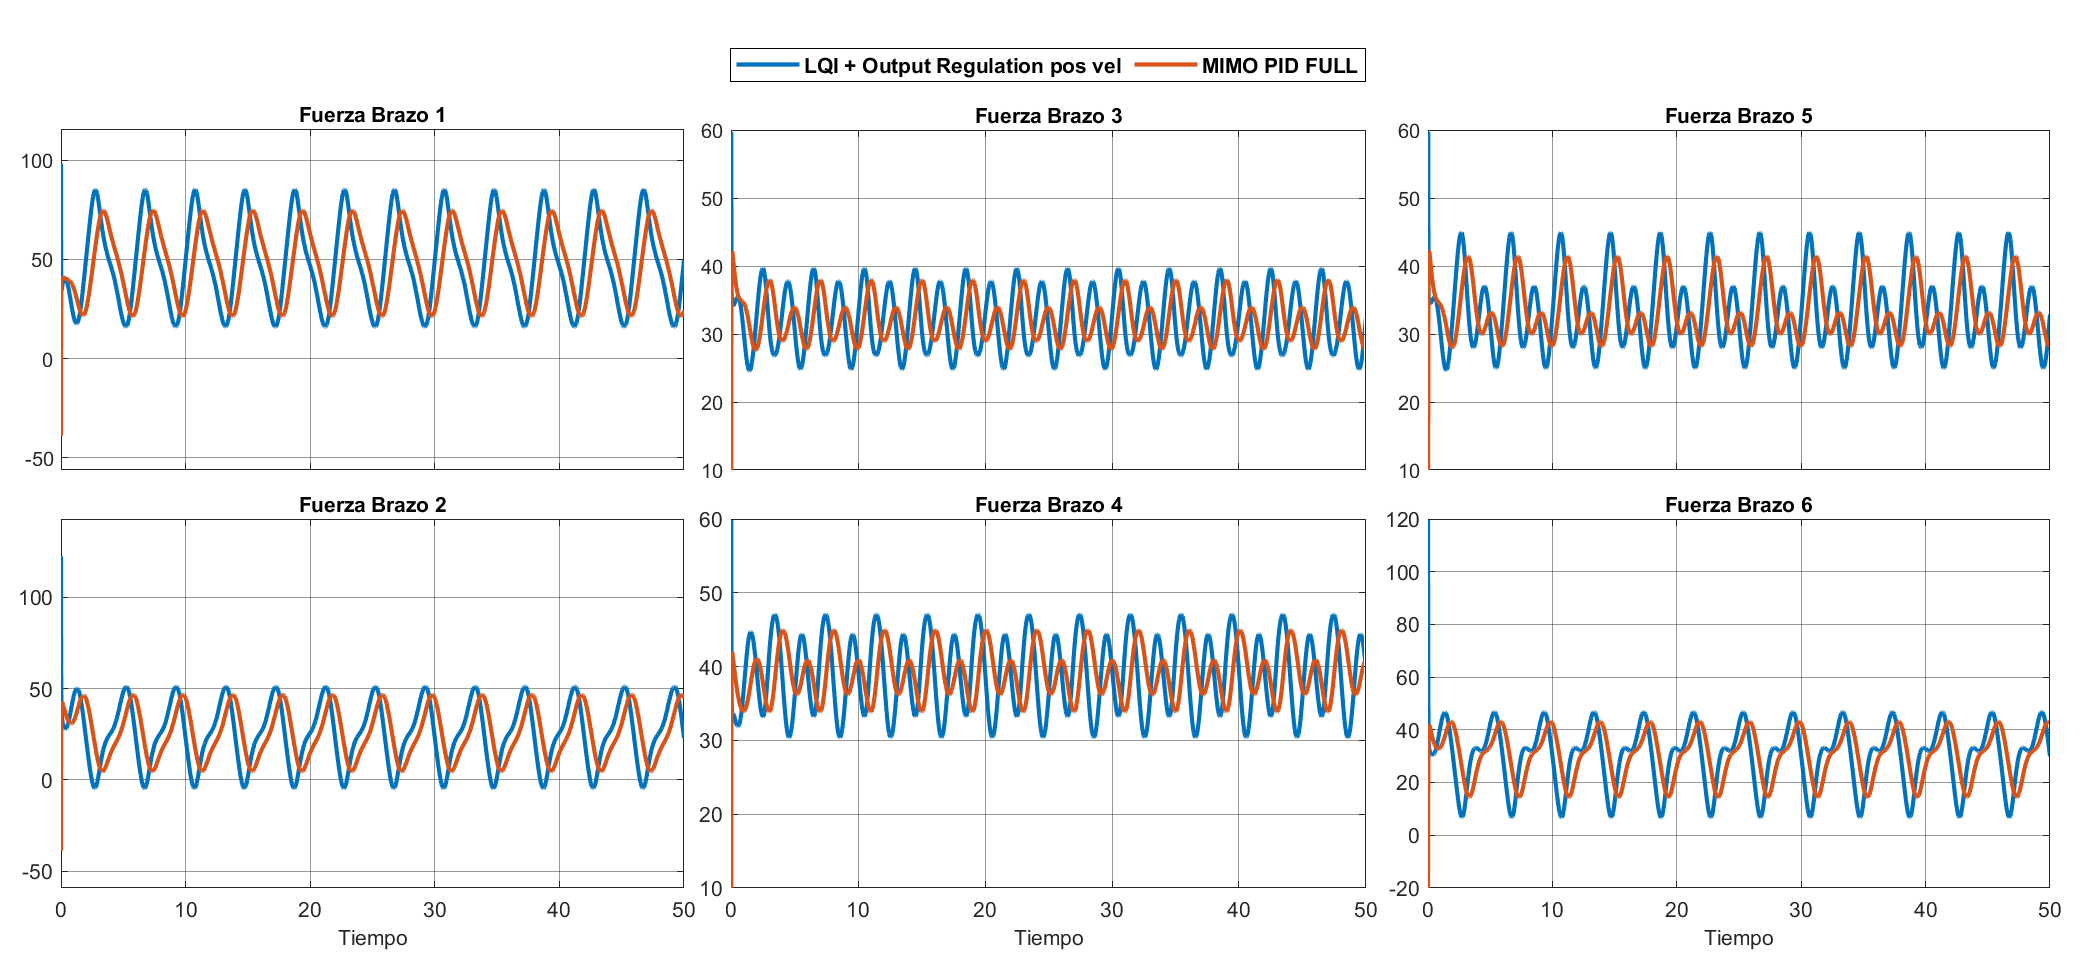
\includegraphics[width=1\columnwidth]{Results/LQI_OR_frec_variable/fuerza_frec_variable.eps}
    \caption{Fuerza de actuación (N) LQI+OR v/s MIMO PID Full, referencia frecuencia variable.}
    \label{fig:lqiOR_fuerza_frec_variable}
\end{figure}

Tanto para las referencias Nro.1 y Nro.2, los errores obtenidos mediante el control LQI con Output Regulation bajaron considerablemente en comparación al controlador MIMO PID Full, evidenciando el efecto del feedforward con la referencia deseada. Se debe notar que, por mucho que se aplica Output Regulation al control, en ninguno de los casos los errores obtenidos son cero. Esto es un punto importante ya que según la definición de Output Regulation garantizaba error cero en estado estacionario. En el caso de la plataforma Stewart, debido a la alta no linealidad que posee, es posible que este sea un factor determinante que impida el error cero en estado estacionario. Otro factor que puede explicar estos resultados, es el no haber pasado las referencias a través del bloque de Cinemática Inversa del capítulo \ref{cap:modeladoStewart}, ya que se tomó como referencia el movimiento de los brazos directamente en lugar de considerar el movimiento de la plataforma superior. Al forzar la trayectoria sin considerar las relaciones dinámicas existentes entre los brazos adyacentes ($1$-$2$ ó $2$-$3$, etc), es posible que se quiera seguir una referencia no realizable, explicando así el error distinto de cero en estado estacionario. Por ejemplo, debido a las condiciones físicas de la plataforma, no es posible tener el brazo 1 en $30(cm)$ de alto mientras el brazo 2 este en $5(cm)$ de alto. Es por esto que, se recomienda asignar el movimiento deseado en la plataforma superior, para posteriormente ser transformado por el bloque de cinemática inversa y así obtener la referencia deseada de los brazos, con el requerimiento necesario de reconocer todos los parámetros de la referencia en su sistema exógeno para poder resolver el problema de Output Regulation en el seguimiento sinusoidal.

Para un análisis más detallado, se consideran nuevamente los índices de desempeño $J_{ISE}$ y $J_u$ de las ecuaciones \ref{eq:indices_desempeño} del capítulo \ref{cap:mimoPID}. El índice $J_{LQI}$ no se considera en esta etapa ya que el controlador MIMO PID al ser sintetizado por control LQI, su costo $J_{LQI}$ es exactamente igual al controlador LQI con Output Regulation, siendo un índice sin información útil para este caso. 

Para un tiempo de simulación $T_{sim}=50(s)$ se muestran los índices de desempeño para la referencia Nro.1 y Nro.2 en la tabla \ref{tab:indices_LQIOR_final}.

\begin{table}[H]
\centering
\begin{tabular}{|c|c|c|c|}
\hline
    \textbf{Referencia} & \textbf{Controlador} & $\mathbf{J_{ISE}}$ & $\mathbf{J_{u}}(\cdot10^5)$ \\ \hline
\multicolumn{1}{|c|}{\multirow{2}{*}{Nro. 1}} &  MIMO PID Full & $1219$ & $3.6337$ \\ \cline{2-4}  
\multicolumn{1}{|c|}{}                        & LQI+OR pos vel & $48.41$ & $3.6347$ \\ \hline
\multicolumn{1}{|c|}{\multirow{2}{*}{Nro. 2}} & MIMO PID Full  & $693.3$ & $4.0638$  \\ \cline{2-4} 
\multicolumn{1}{|c|}{}                        & LQI+OR pos vel & $50.37$ & $4.2358$  \\ \hline
\end{tabular}
\caption{Desempeño para LQI con Output Regulation posición velocidad y PID MIMO Full, referencias sinusoidales de frecuencia fija (Nro.1) y variable (Nro.2).}
\label{tab:indices_LQIOR_final}
\end{table}

De la tabla \ref{tab:indices_LQIOR_final} anterior podemos notar la mejoría significativa lograda con el problema de Output Regulation. Considerando los índices del controlador MIMO PID Full como referencia, el controlador LQI con Output Regulation posee una disminución del $96.0\%$ para el $J_{ISE}$ y un aumento del $0.02\%$ del $J_u$ para la referencia Nro.1. Por otro lado para la referencia Nro.2, el controlador LQI con Output Regulation obtiene una disminución del $92.7\%$ de la integral del error cuadrático $J_{ISE}$ y un aumento del $4.2\%$ del esfuerzo de control $J_u$. Esto refleja lo mostrado en las gráficas anteriores, donde se logró disminuir considerablemente el error de seguimiento a costa de un leve aumento en la fuerza de actuación de los brazos.\\

Con los resultados anteriores obtenidos, se debe hacer mención de los 3 puntos más importantes mejorados con la prepuesta de control realizada:
\begin{itemize}
    \item Capacidad de seguimiento sinusoidal gracias al feedforward aplicado con el problema de Output Regulation.
    \item Aumento de la precisión del seguimiento sinusoidal al incluir la velocidad como parte de la referencia en el problema de Output Regulation de la plataforma Stewart.
    \item Eliminación de cualquier componente constante en el error de seguimiento, gracias al integrador implementado en el control LQI, garantizando error estacionario cero para componentes constantes en la referencia.
\end{itemize}